% Faithful LaTeX/Beamer reconstruction of Department PINN Presentation.pdf
% Content, order, titles, tables, and figures follow the 20-slide source deck.
\documentclass[aspectratio=169,11pt]{beamer}

\usepackage{fontspec}
\usepackage{microtype}
\usepackage{graphicx}
\usepackage{booktabs}
\usepackage{tabularx}
\usepackage{array}
\usepackage{colortbl}
\usepackage{mathtools}
\usepackage{hyperref}

\setsansfont{Avenir Next}[Ligatures=TeX]
\setmainfont{Avenir Next}[Ligatures=TeX]
\setmonofont{Menlo}

\definecolor{Paper}{HTML}{F7F6F3}
\definecolor{Canvas}{HTML}{FFFFFF}
\definecolor{Ink}{HTML}{152A3A}
\definecolor{Muted}{HTML}{65737B}
\definecolor{Garnet}{HTML}{9C2745}
\definecolor{Teal}{HTML}{2D7C73}
\definecolor{Cobalt}{HTML}{315B7D}
\definecolor{Line}{HTML}{D7DDDF}
\definecolor{Tint}{HTML}{E9EFF1}
\definecolor{TintWarm}{HTML}{F1E8EB}

\setbeamercolor{normal text}{fg=Ink,bg=Paper}
\setbeamercolor{frametitle}{fg=Ink,bg=Paper}
\setbeamercolor{structure}{fg=Garnet}
\setbeamercolor{itemize item}{fg=Garnet}
\setbeamercolor{itemize subitem}{fg=Teal}
\setbeamercolor{alerted text}{fg=Garnet}
\setbeamerfont{frametitle}{series=\bfseries,size=\fontsize{15.5}{18.2}}
\setbeamerfont{normal text}{size=\fontsize{11}{14}}

\setbeamersize{text margin left=0.68cm,text margin right=0.68cm}
\setbeamertemplate{navigation symbols}{}
\setbeamertemplate{footline}{}
\setbeamertemplate{headline}{}
\setbeamertemplate{background canvas}{\color{Paper}\rule{\paperwidth}{\paperheight}}
\setbeamertemplate{itemize item}{\raisebox{0.34ex}{\textcolor{Garnet}{\rule{0.10cm}{0.10cm}}}}
\setbeamertemplate{itemize subitem}{\raisebox{0.40ex}{\textcolor{Teal}{\rule{0.075cm}{0.075cm}}}}
\setbeamertemplate{frametitle}{%
  \nointerlineskip
  \begin{beamercolorbox}[wd=\paperwidth,ht=0.76cm,dp=0.20cm,leftskip=0.68cm,rightskip=0.68cm]{frametitle}
    \usebeamerfont{frametitle}\insertframetitle
  \end{beamercolorbox}
  \vspace{-0.08cm}
  \hspace{0.68cm}%
  \textcolor{Garnet}{\rule{0.54cm}{1.55pt}}\hspace{0.05cm}%
  \textcolor{Teal}{\rule{0.26cm}{1.55pt}}\hspace{0.09cm}%
  \textcolor{Line}{\rule{12.83cm}{0.50pt}}
}

\setlength{\fboxsep}{2.1pt}
\setlength{\fboxrule}{0.45pt}
\newcommand{\imagepanel}[2][]{\fcolorbox{Line}{Canvas}{\includegraphics[#1]{#2}}}
\newcommand{\regimepair}[2]{\textbf{#1}\par{\footnotesize\color{Muted}#2}}

\title{Physics-Informed Neural Network for a Reduced WNT-HOX-Retinoic Acid Model of Colorectal Cancer}
\author{Amirkhan Aidarkhan \and Nathaniel Kim}
\date{July 21, 2026}

\begin{document}

% 1 — Title
\begin{frame}[plain]
  \vspace{0.14cm}
  \begin{columns}[T,totalwidth=\textwidth]
    \begin{column}{0.18\textwidth}
      
\includegraphics[width=\linewidth]{assets/source_swarthmore_logo.jpg}
    \end{column}
    \begin{column}{0.78\textwidth}
      {\fontsize{20}{23}\selectfont\bfseries\color{Ink}\inserttitle\par}
      \vspace{0.22cm}
      {\small\bfseries\color{Garnet}Amirkhan Aidarkhan, Nathaniel Kim}\par
      {\small\color{Muted}Advisor: Dr. Kataboh}\par
      \vspace{0.20cm}
      {\scriptsize\color{Muted}Department of Mathematics \& Statistics, Swarthmore College \hfill July 21, 2026}
    \end{column}
  \end{columns}
  \vspace{0.32cm}
  \begin{columns}[c,totalwidth=0.88\textwidth]
    \begin{column}{0.39\textwidth}
      \centering\imagepanel[height=3.00cm]{assets/source_colon_cancer.jpg}
    \end{column}
    \begin{column}{0.08\textwidth}
      \centering{\LARGE\bfseries\color{Garnet}+}
    \end{column}
    \begin{column}{0.39\textwidth}
      \centering\imagepanel[height=2.82cm]{assets/source_neural_network.jpg}
    \end{column}
  \end{columns}
\end{frame}

% 2 — Overview
\begin{frame}{Overview}
  \vspace{0.38cm}
  \begin{itemize}\setlength\itemsep{0.28cm}
    \item Biology/Schematic
    \item Equations
    \item Forward PINN
    \item Inverse PINN
    \item Inverse Bayesian PINN
    \item Next Steps
  \end{itemize}
\end{frame}

% 3 — Biological network
\begin{frame}{Biological Network Governing WNT--HOX--RA Signaling}
  \small
  \textbf{\color{Garnet}Objective}\par
  \vspace{0.08cm}
  Develop a reduced mathematical model describing the interactions among the WNT, HOX, and Retinoic Acid (RA) pathways during colorectal cancer progression.
  \vspace{0.20cm}
  \begin{columns}[T,totalwidth=\textwidth]
    \begin{column}{0.48\textwidth}
      \centering\imagepanel[height=4.15cm]{assets/source_biological_network.jpg}
    \end{column}
    \begin{column}{0.47\textwidth}
      \textbf{\color{Garnet}State Variables}\par
      \vspace{0.08cm}
      $\mathbf y=[B(t),P(t),H_5(t),H_{13}(t),M(t),R(t),C(t)]$\par
      \vspace{0.18cm}
      \begin{tabular}{@{}>{$}l<{$}@{\hspace{0.45cm}}l@{}}
        B & $\beta$-catenin \\
        P & APC \\
        H_5 & HOXA5 \\
        H_{13} & HOXA13 \\
        M & MYC \\
        R & Retinoic Acid \\
        C & CYP26A1
      \end{tabular}
    \end{column}
  \end{columns}
\end{frame}

% 4 — RA input
\begin{frame}{RA Input + Treatment}
  \begin{columns}[T,totalwidth=\textwidth]
    \begin{column}{0.48\textwidth}
      \centering
      \textbf{\color{Cobalt}RA Input}\par\vspace{0.12cm}
      \imagepanel[width=0.96\linewidth]{assets/source_ra_input.jpg}
      \vspace{0.20cm}
      {\large$A_d\!\left[1+\cos\!\left(\dfrac{2\pi t}{T_d}-\phi\right)\right]$}
    \end{column}
    \begin{column}{0.48\textwidth}
      \centering
      \textbf{\color{Cobalt}ATRA Treatment}\par\vspace{0.12cm}
      \imagepanel[width=0.96\linewidth]{assets/source_atra_treatment.jpg}
      \vspace{0.20cm}
      {\large$u_R(t)=\dfrac{D}{2}\!\left[\tanh q(t-t_1)-\tanh q(t-t_2)\right]$}
    \end{column}
  \end{columns}
\end{frame}

% 5 — Model equations
\begin{frame}{Dimensional Model}
  \centering
  \imagepanel[height=6.15cm]{assets/source_dimensional_model.jpg}
\end{frame}

% 6 — Four regimes + supplied image
\begin{frame}{4 Regimes}
  \begin{columns}[T,totalwidth=\textwidth]
    \begin{column}{0.43\textwidth}
      \small
      Disease progression is modeled by increasing WNT signaling ($W$) and progressive loss of APC function ($\theta_P$), mimicking CRC progression.
      \vspace{0.22cm}
      \begin{itemize}\setlength\itemsep{0.10cm}
        \item ``Normal''
          \begin{itemize}\item $W=0.8$, $\theta_P=1.0$\end{itemize}
        \item ``Early Adenoma''
          \begin{itemize}\item $W=1.0$, $\theta_P=0.75$\end{itemize}
        \item ``Advanced Adenoma''
          \begin{itemize}\item $W=1.5$, $\theta_P=0.5$\end{itemize}
        \item ``Severe APC Loss''
          \begin{itemize}\item $W=2.0$, $\theta_P=0.25$\end{itemize}
      \end{itemize}
    \end{column}
    \begin{column}{0.54\textwidth}
      \vspace{0.42cm}
      \centering
      \imagepanel[width=0.96\linewidth]{assets/colorectal_progression.png}
    \end{column}
  \end{columns}
\end{frame}

% 7 — Reference dynamics
\begin{frame}[plain]
  \centering
  \vspace{0.38cm}
  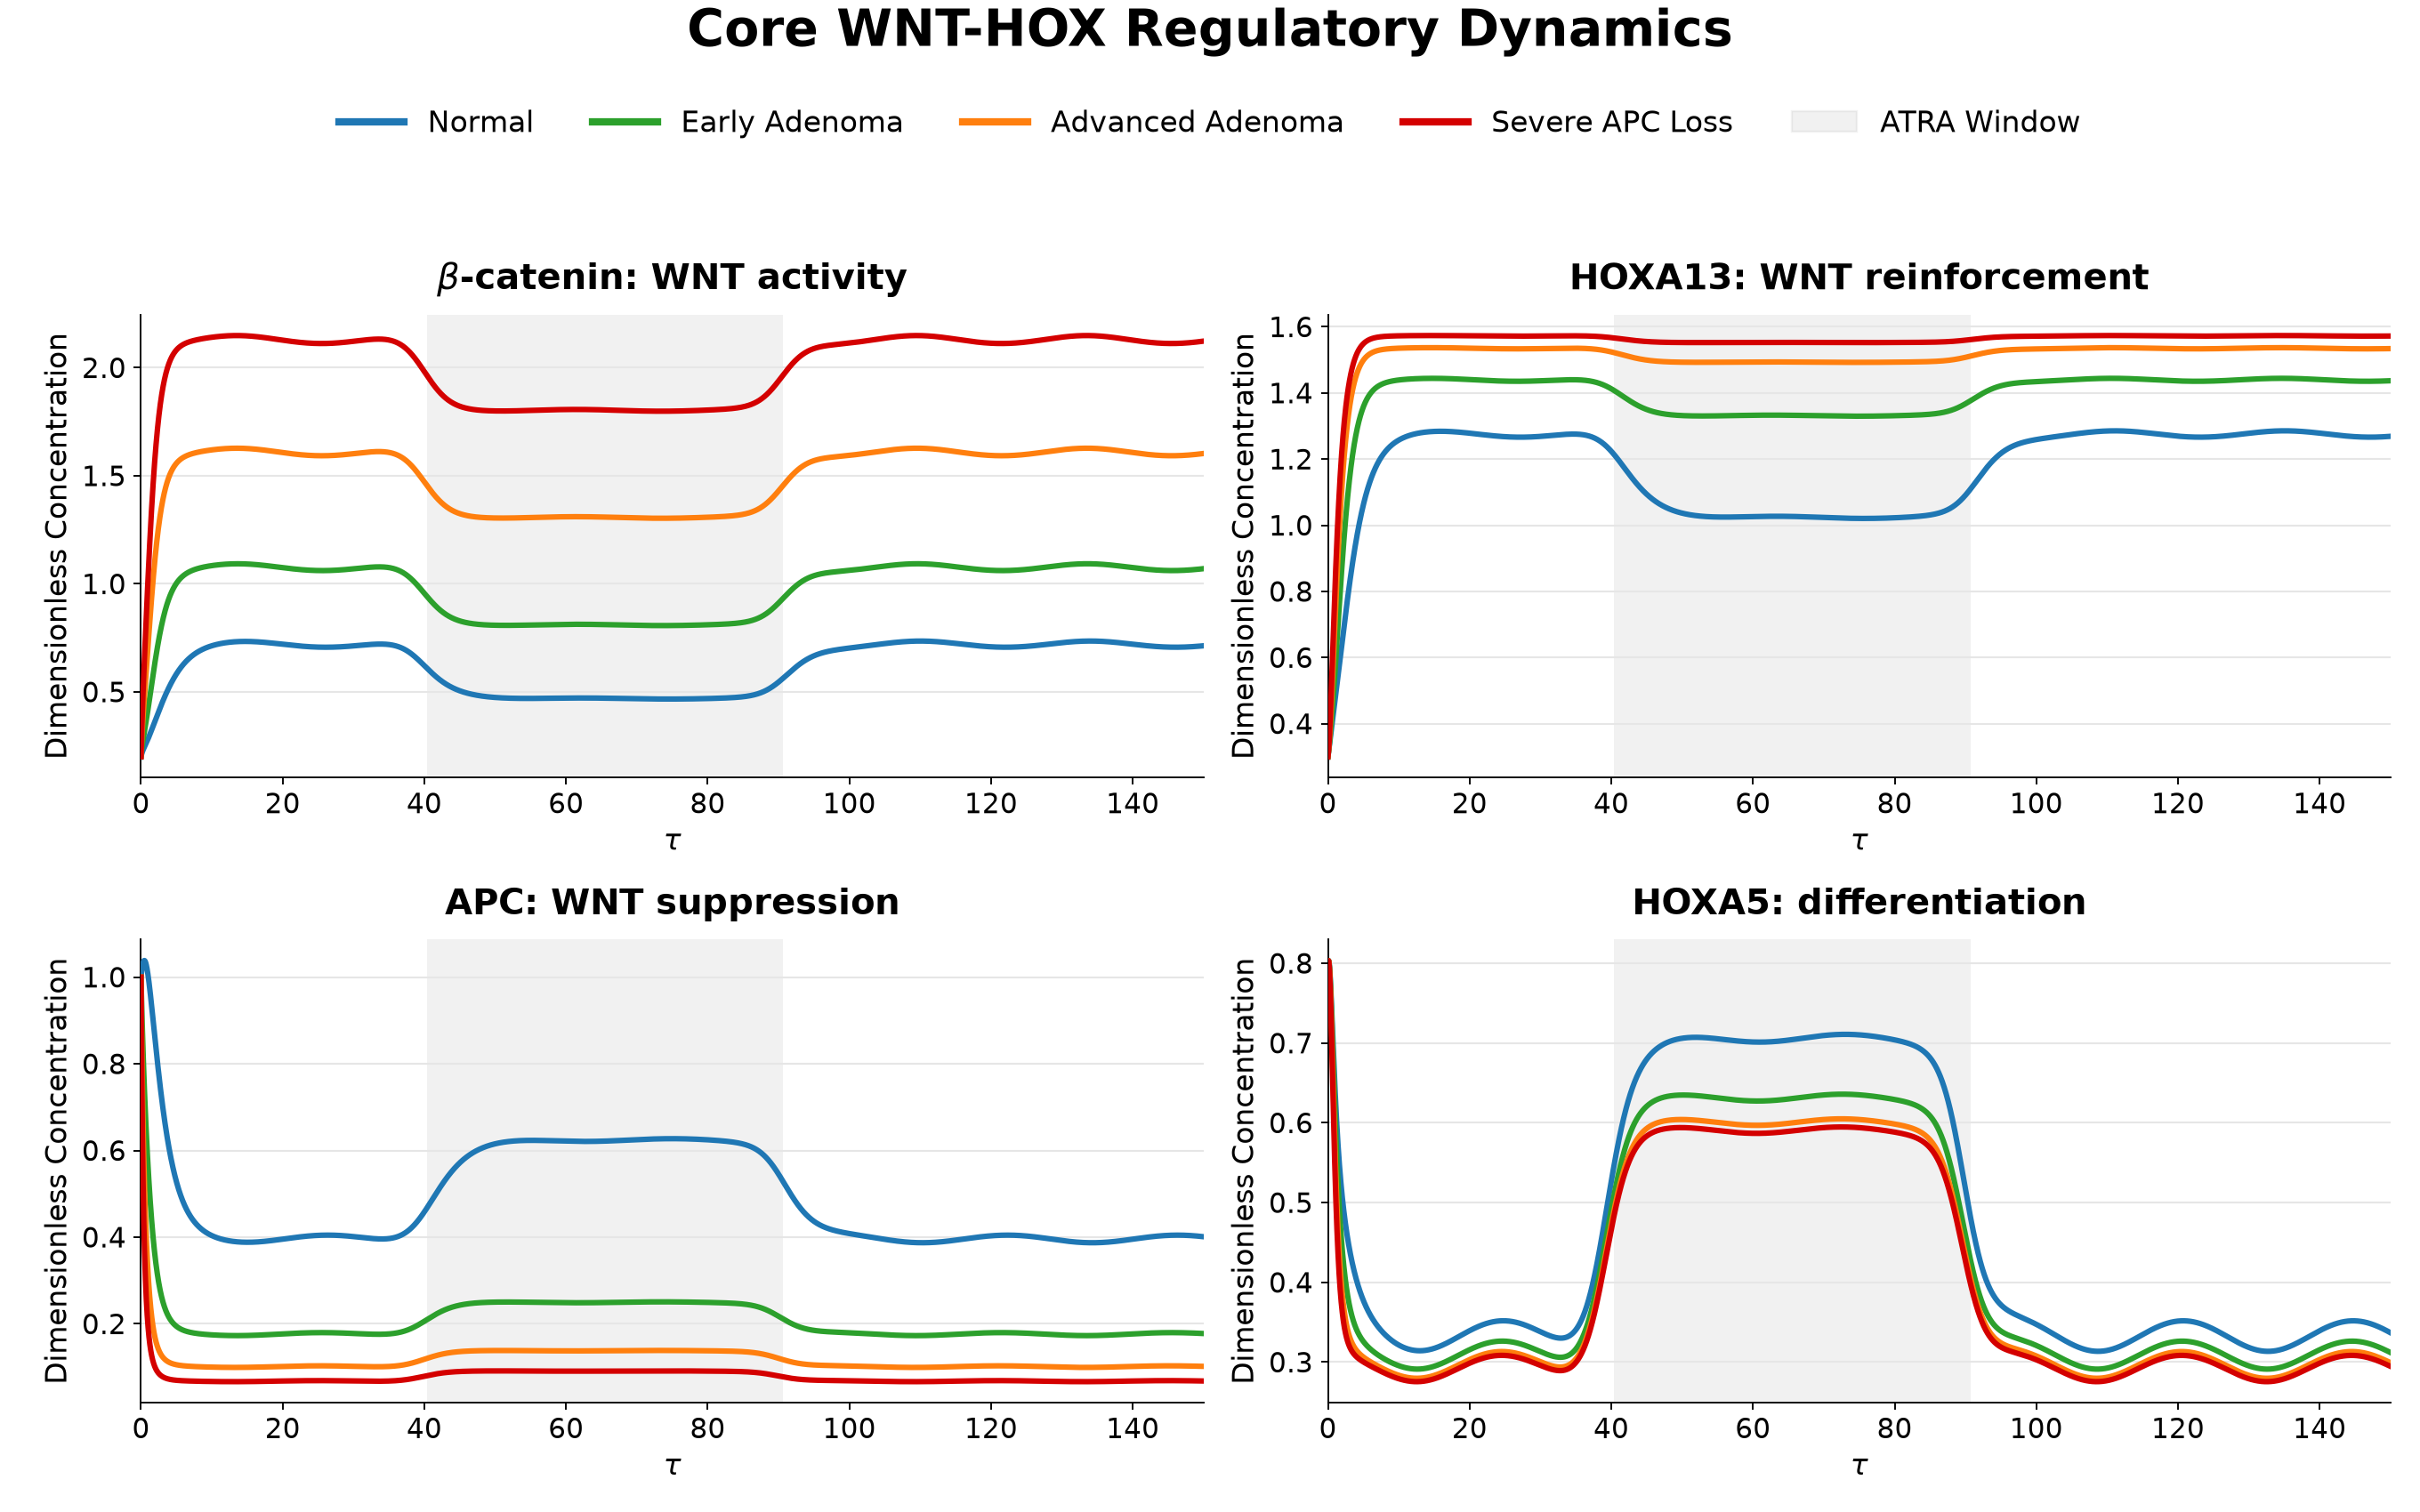
\includegraphics[height=8.12cm]{assets/scipy_core_dynamics.png}
\end{frame}

% 8 — Forward PINN architecture
\begin{frame}[plain]
  \centering
  \vspace{0.34cm}
  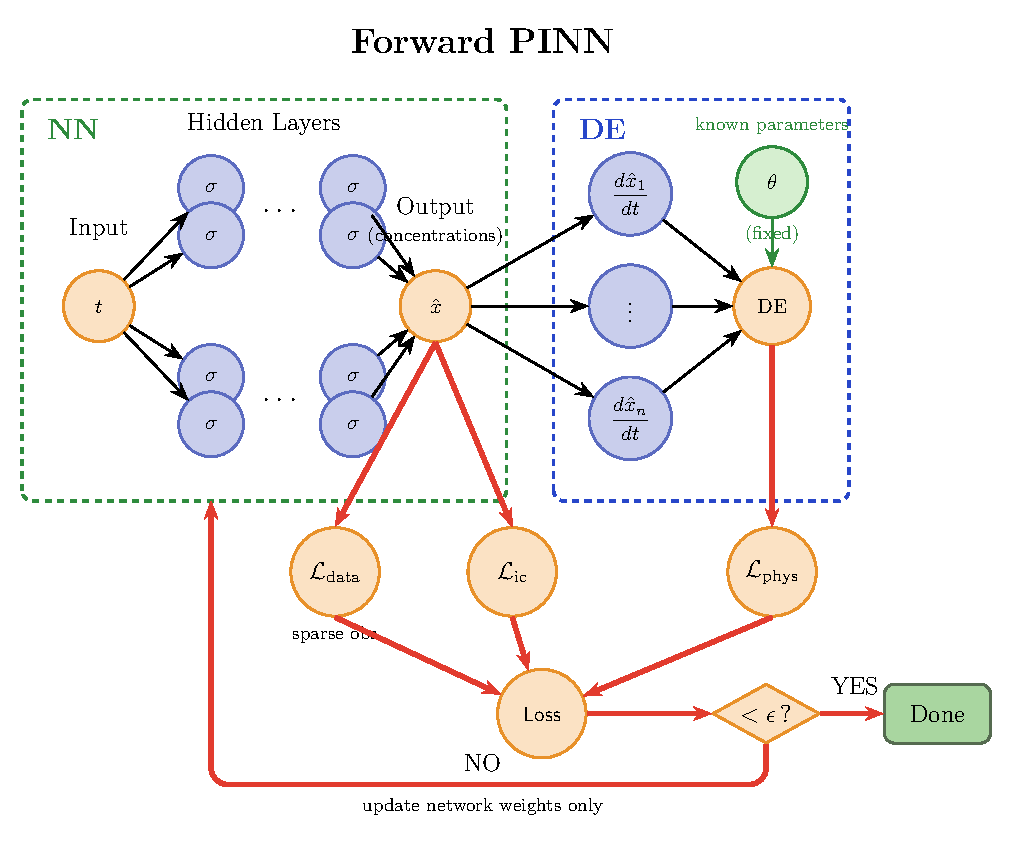
\includegraphics[height=8.20cm]{assets/forward_architecture.pdf}
\end{frame}

% 9 — Forward loss
\begin{frame}{Forward PINN Loss}
  \centering
  \vspace{0.06cm}
  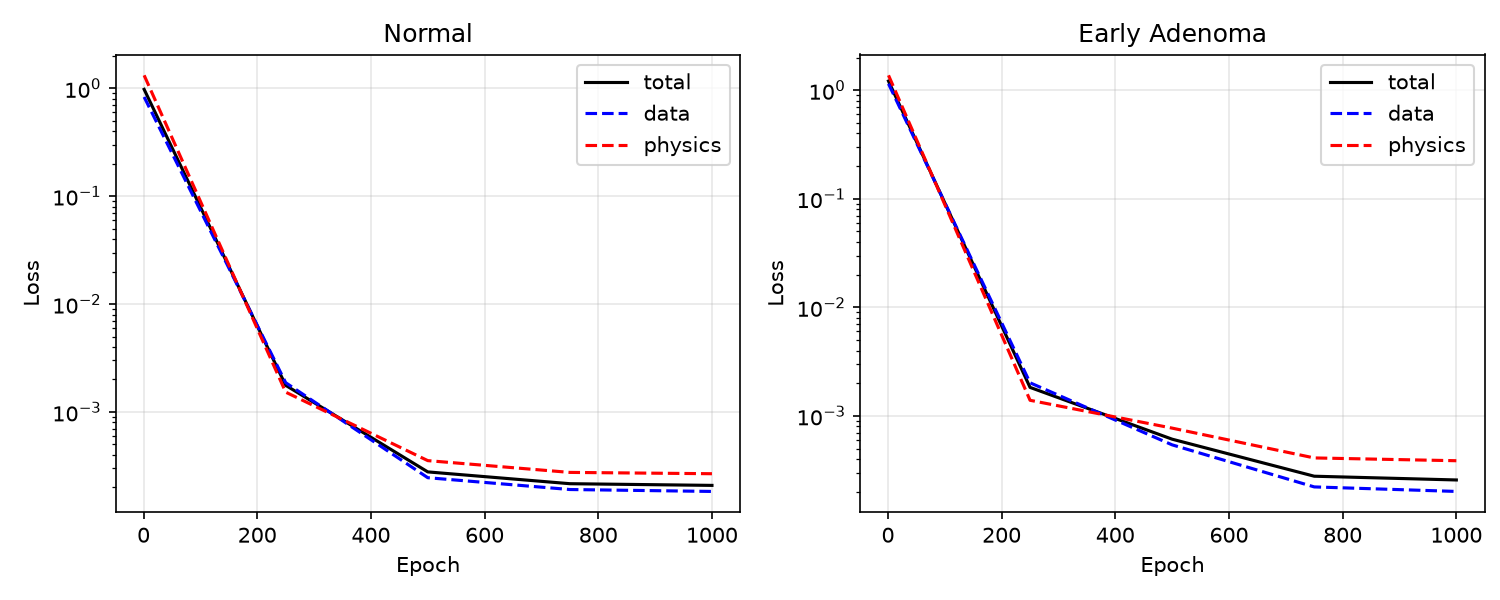
\includegraphics[width=0.59\textwidth]{assets/forward_losses_top.png}\par
  \vspace{0.08cm}
  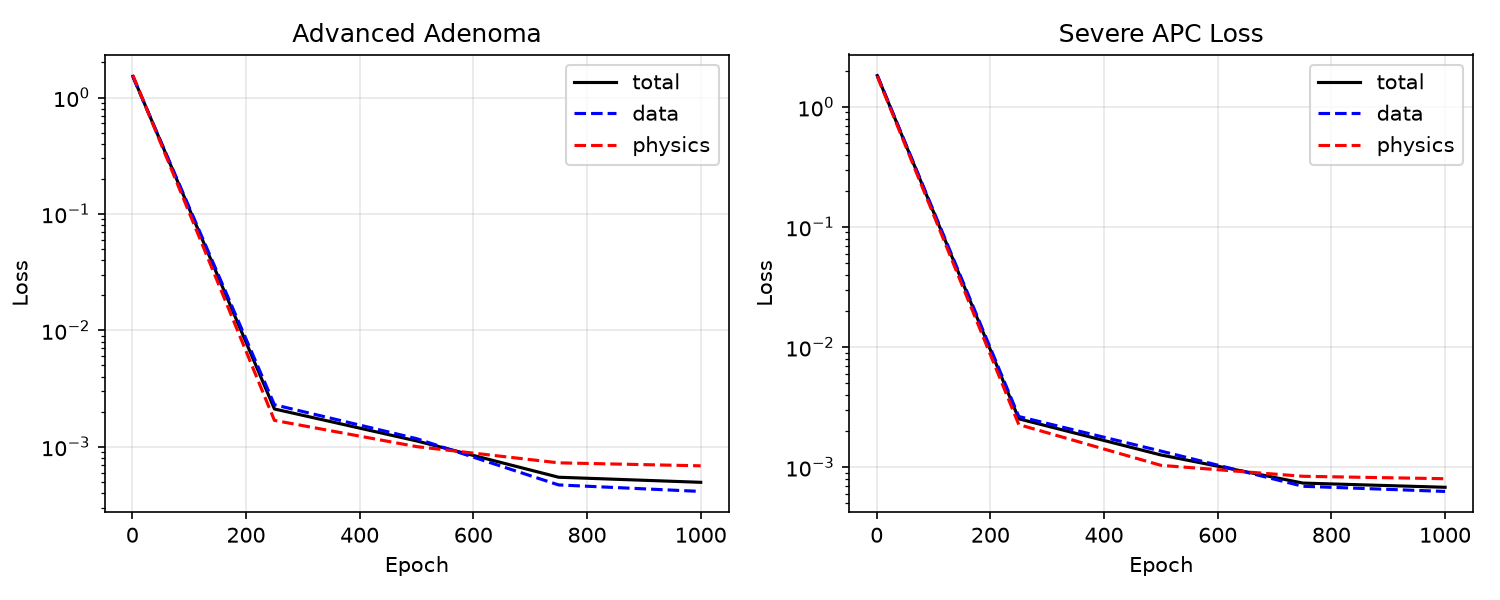
\includegraphics[width=0.59\textwidth]{assets/forward_losses_bottom.png}
\end{frame}

% 10 — Forward trajectories
\begin{frame}[plain]
  \centering
  \vspace{0.38cm}
  
\includegraphics[height=8.12cm]{assets/pinn_forward_core_dynamics.png}
\end{frame}

% 11 — Inverse PINN architecture
\begin{frame}[plain]
  \centering
  \vspace{0.34cm}
  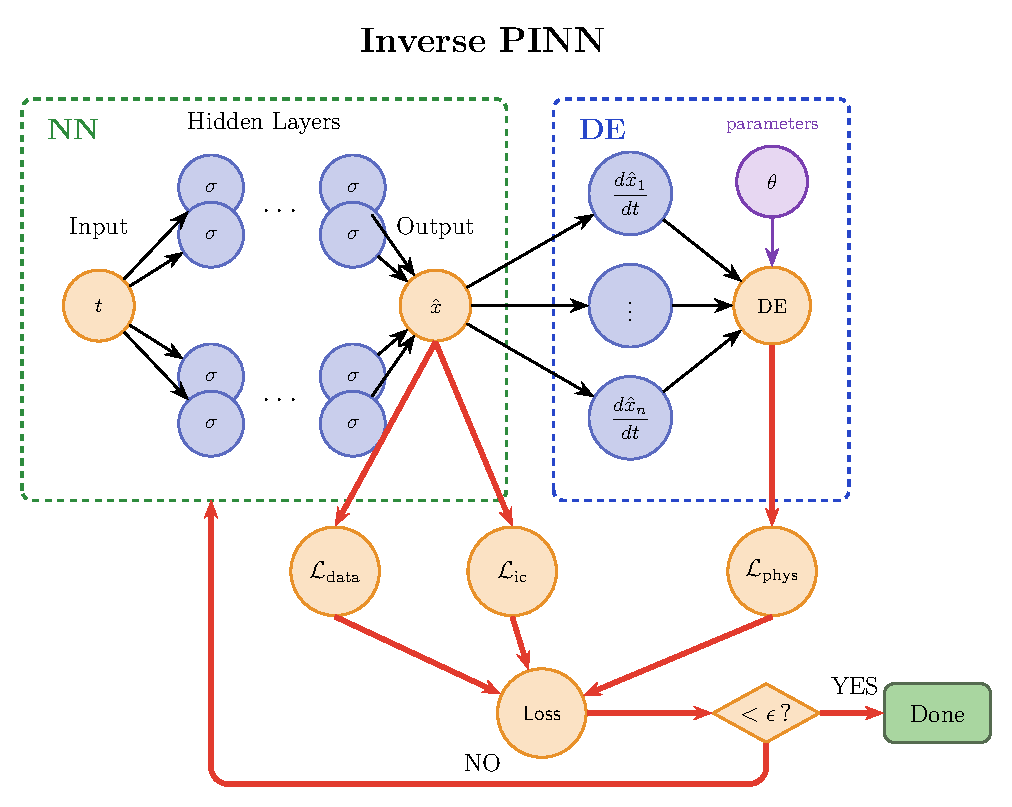
\includegraphics[height=8.20cm]{assets/inverse_architecture.pdf}
\end{frame}

% 12 — Inverse loss
\begin{frame}{Inverse PINN Loss}
  \centering
  \vspace{0.06cm}
  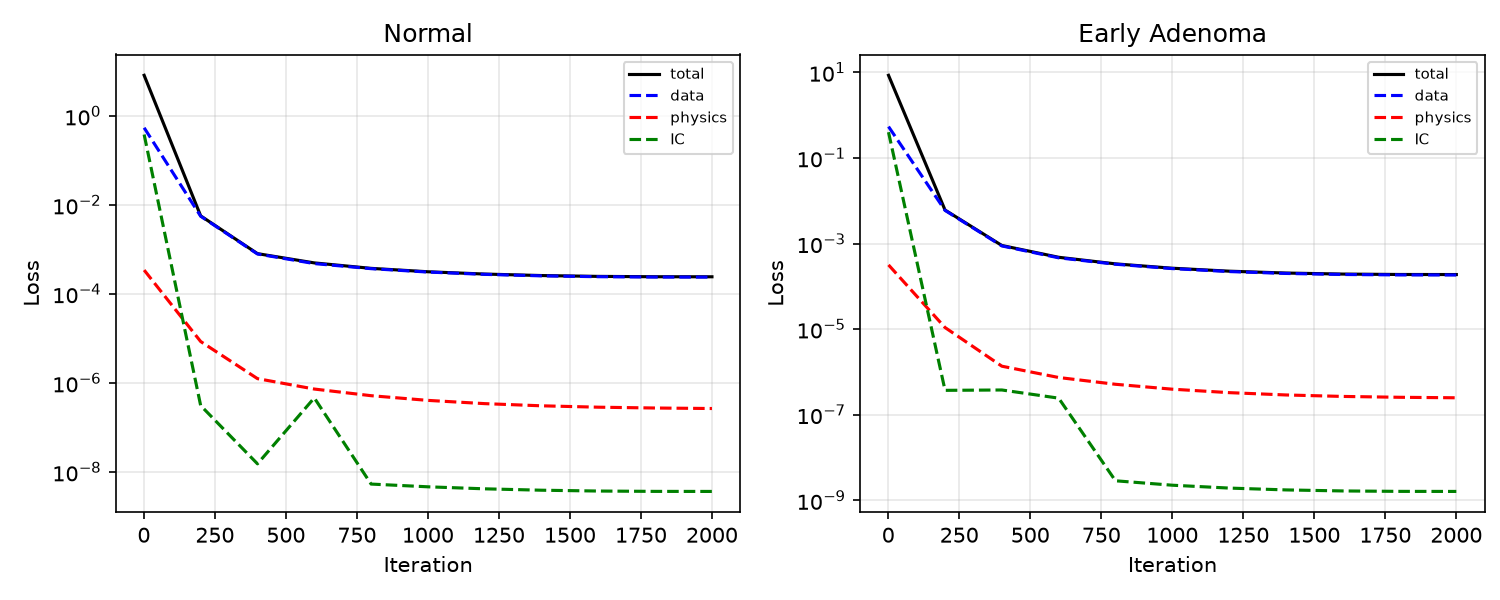
\includegraphics[width=0.59\textwidth]{assets/inverse_losses_top.png}\par
  \vspace{0.08cm}
  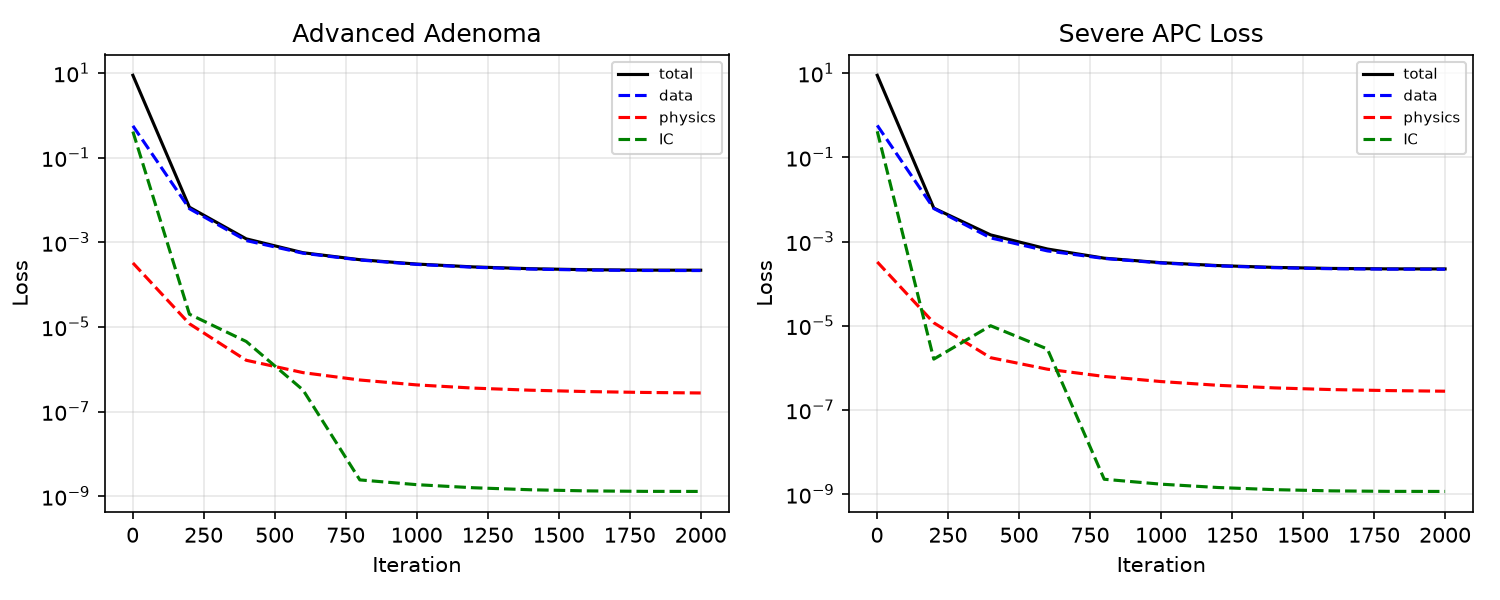
\includegraphics[width=0.59\textwidth]{assets/inverse_losses_bottom.png}
\end{frame}

% 13 — Inverse trajectories
\begin{frame}[plain]
  \centering
  \vspace{0.38cm}
  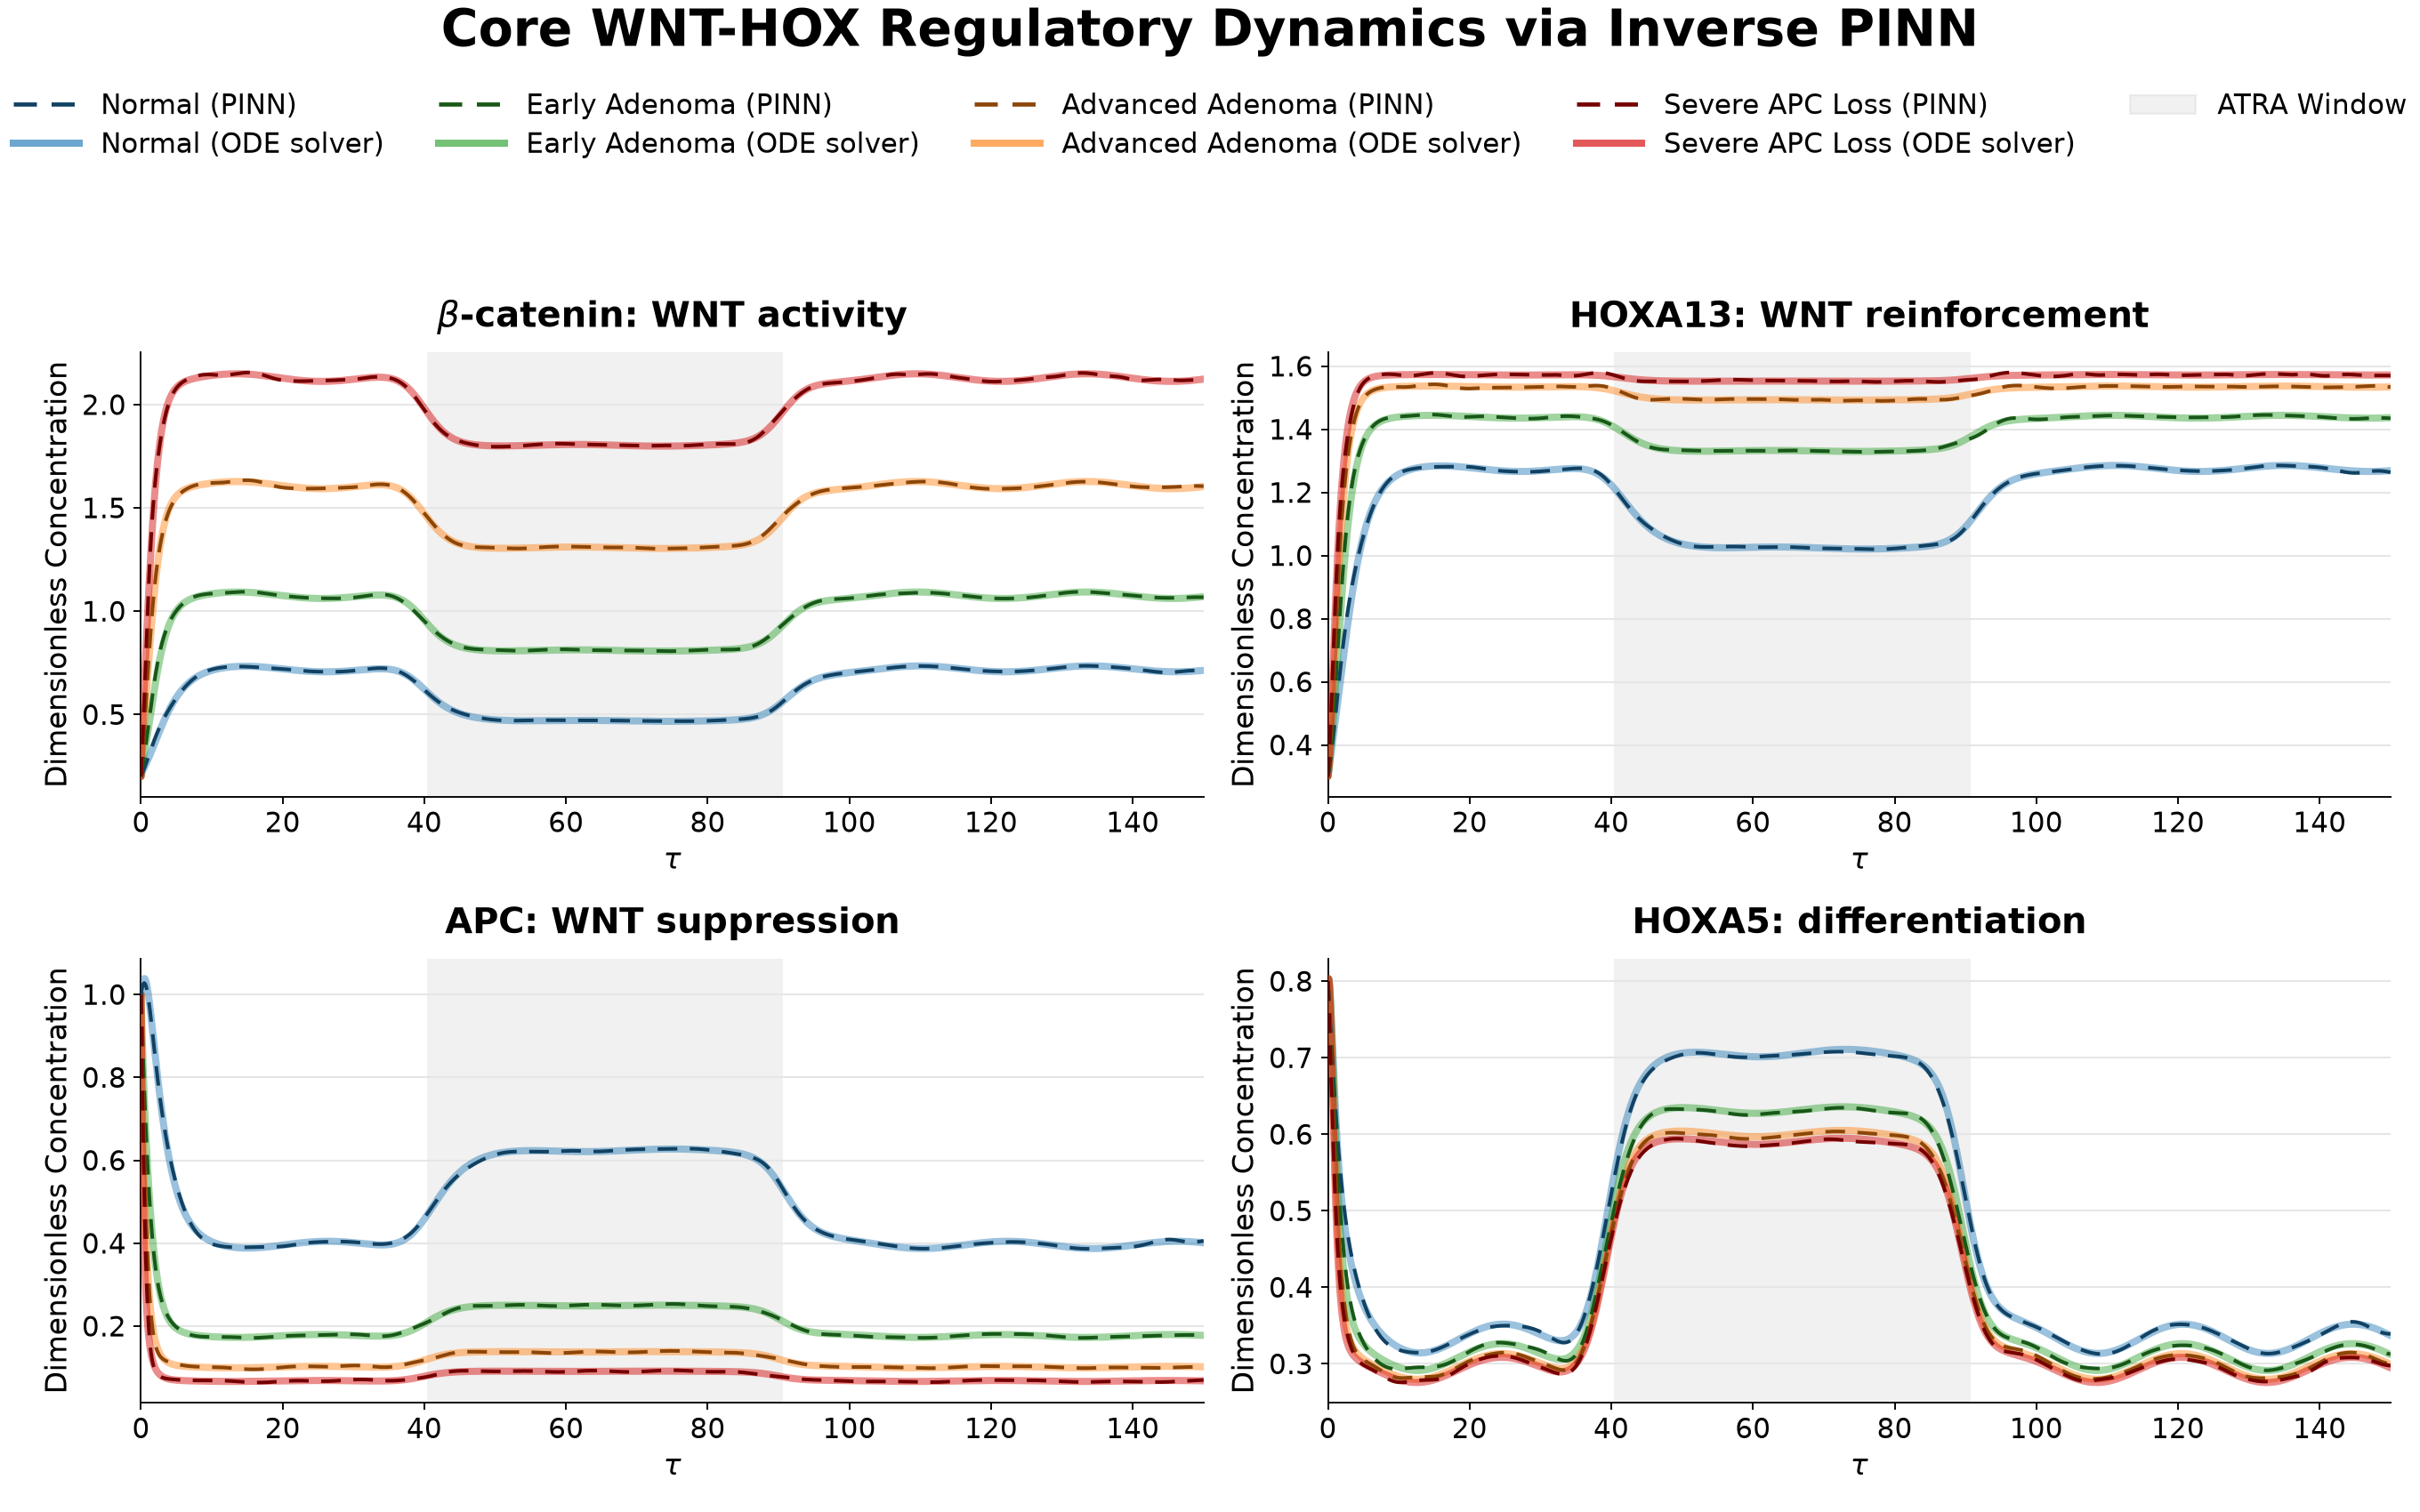
\includegraphics[height=8.12cm]{assets/pinn_inverse_core_dynamics.png}
\end{frame}

% 14 — Parameter recovery bars
\begin{frame}[plain]
  \centering
  \vspace{0.35cm}
  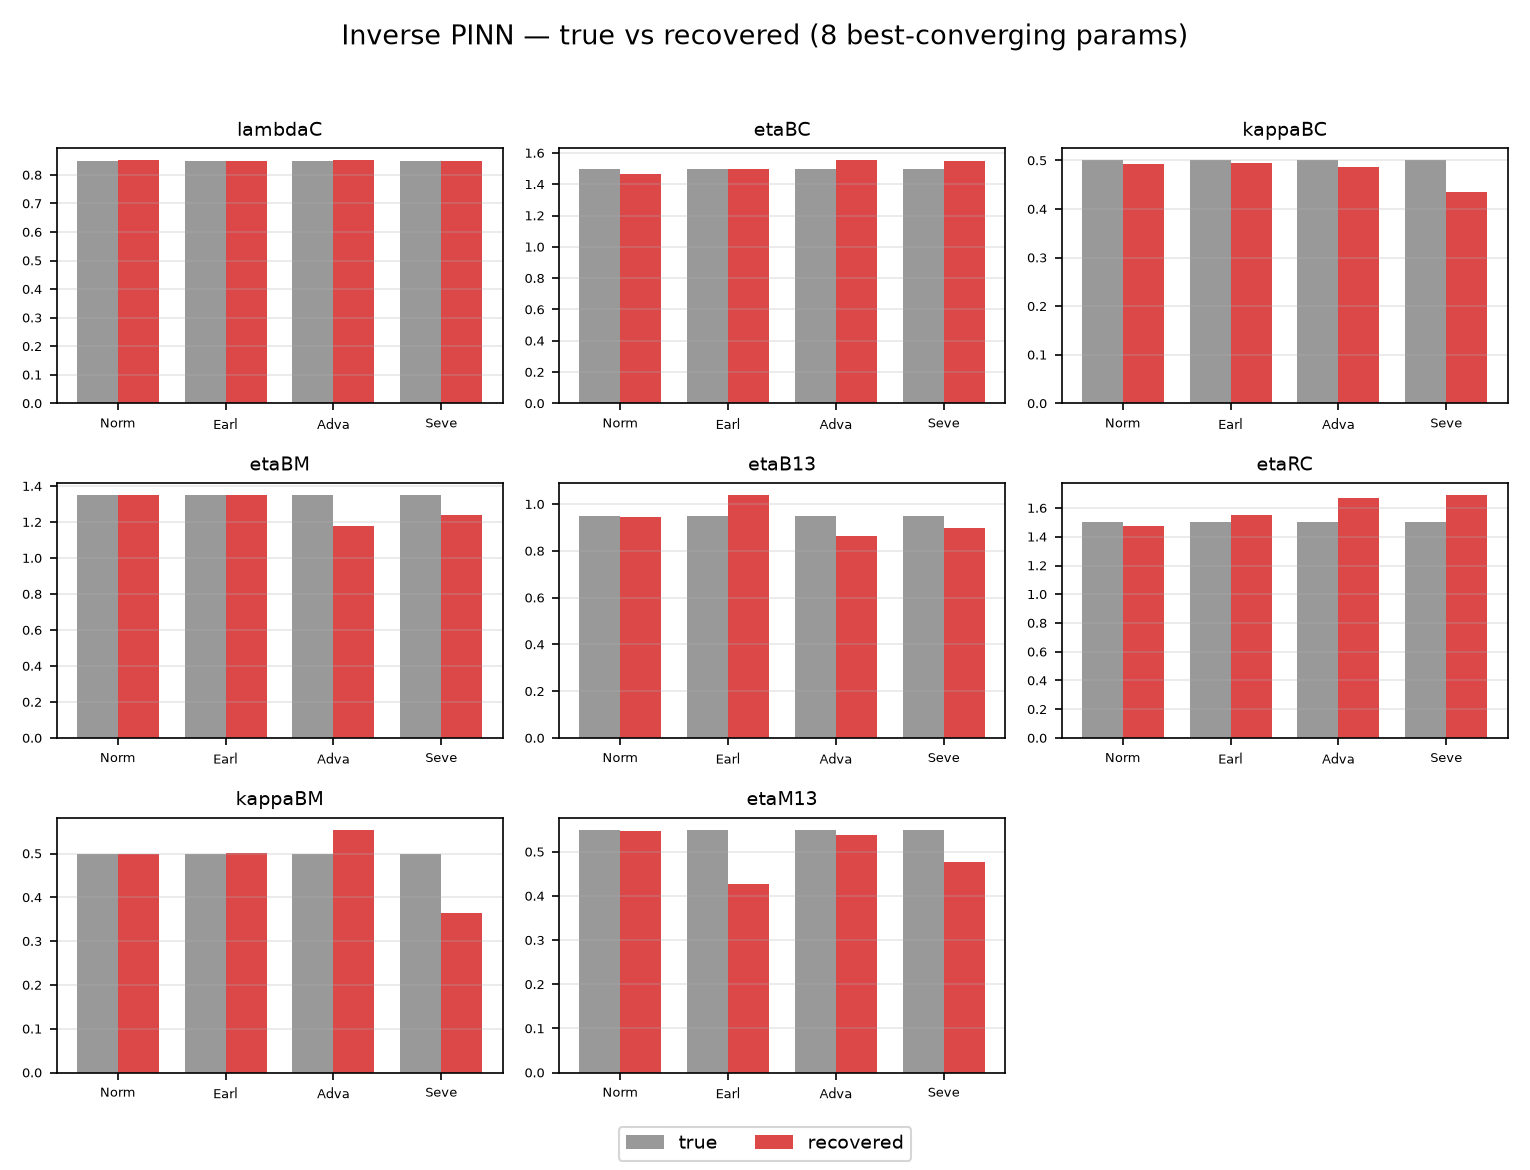
\includegraphics[height=8.18cm]{assets/inverse_recovery_bars_best8.png}
\end{frame}

% 15 — Bayesian normal
\begin{frame}{Inverse Bayesian PINN - uncertainty quantification}
  \centering
  \vspace{0.20cm}
  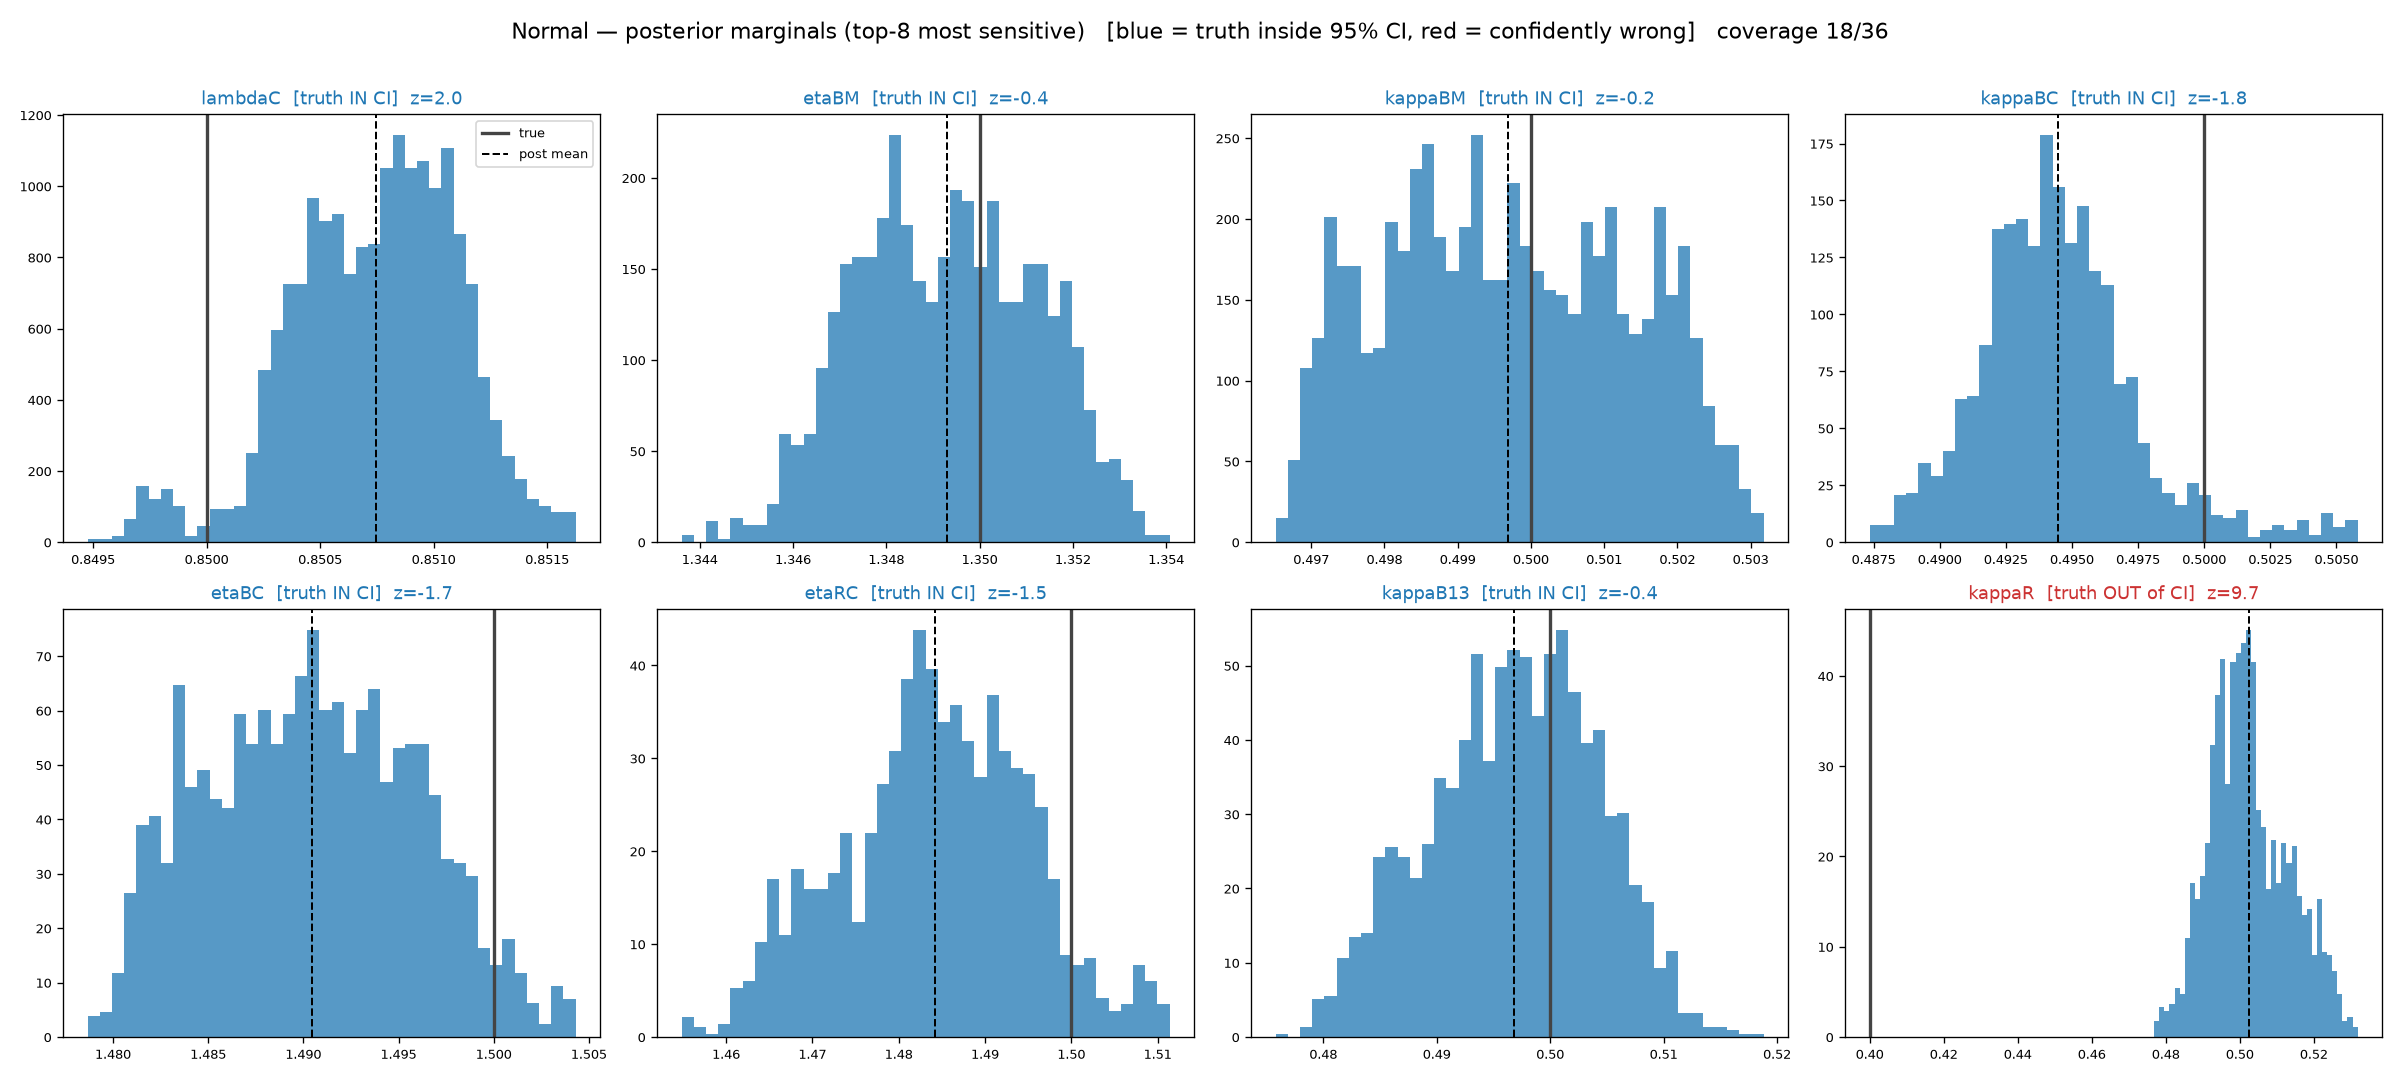
\includegraphics[width=0.96\textwidth]{assets/normal_top8_marginals.png}
\end{frame}

% 16 — Bayesian severe
\begin{frame}[plain]
  \centering
  \vspace{1.02cm}
  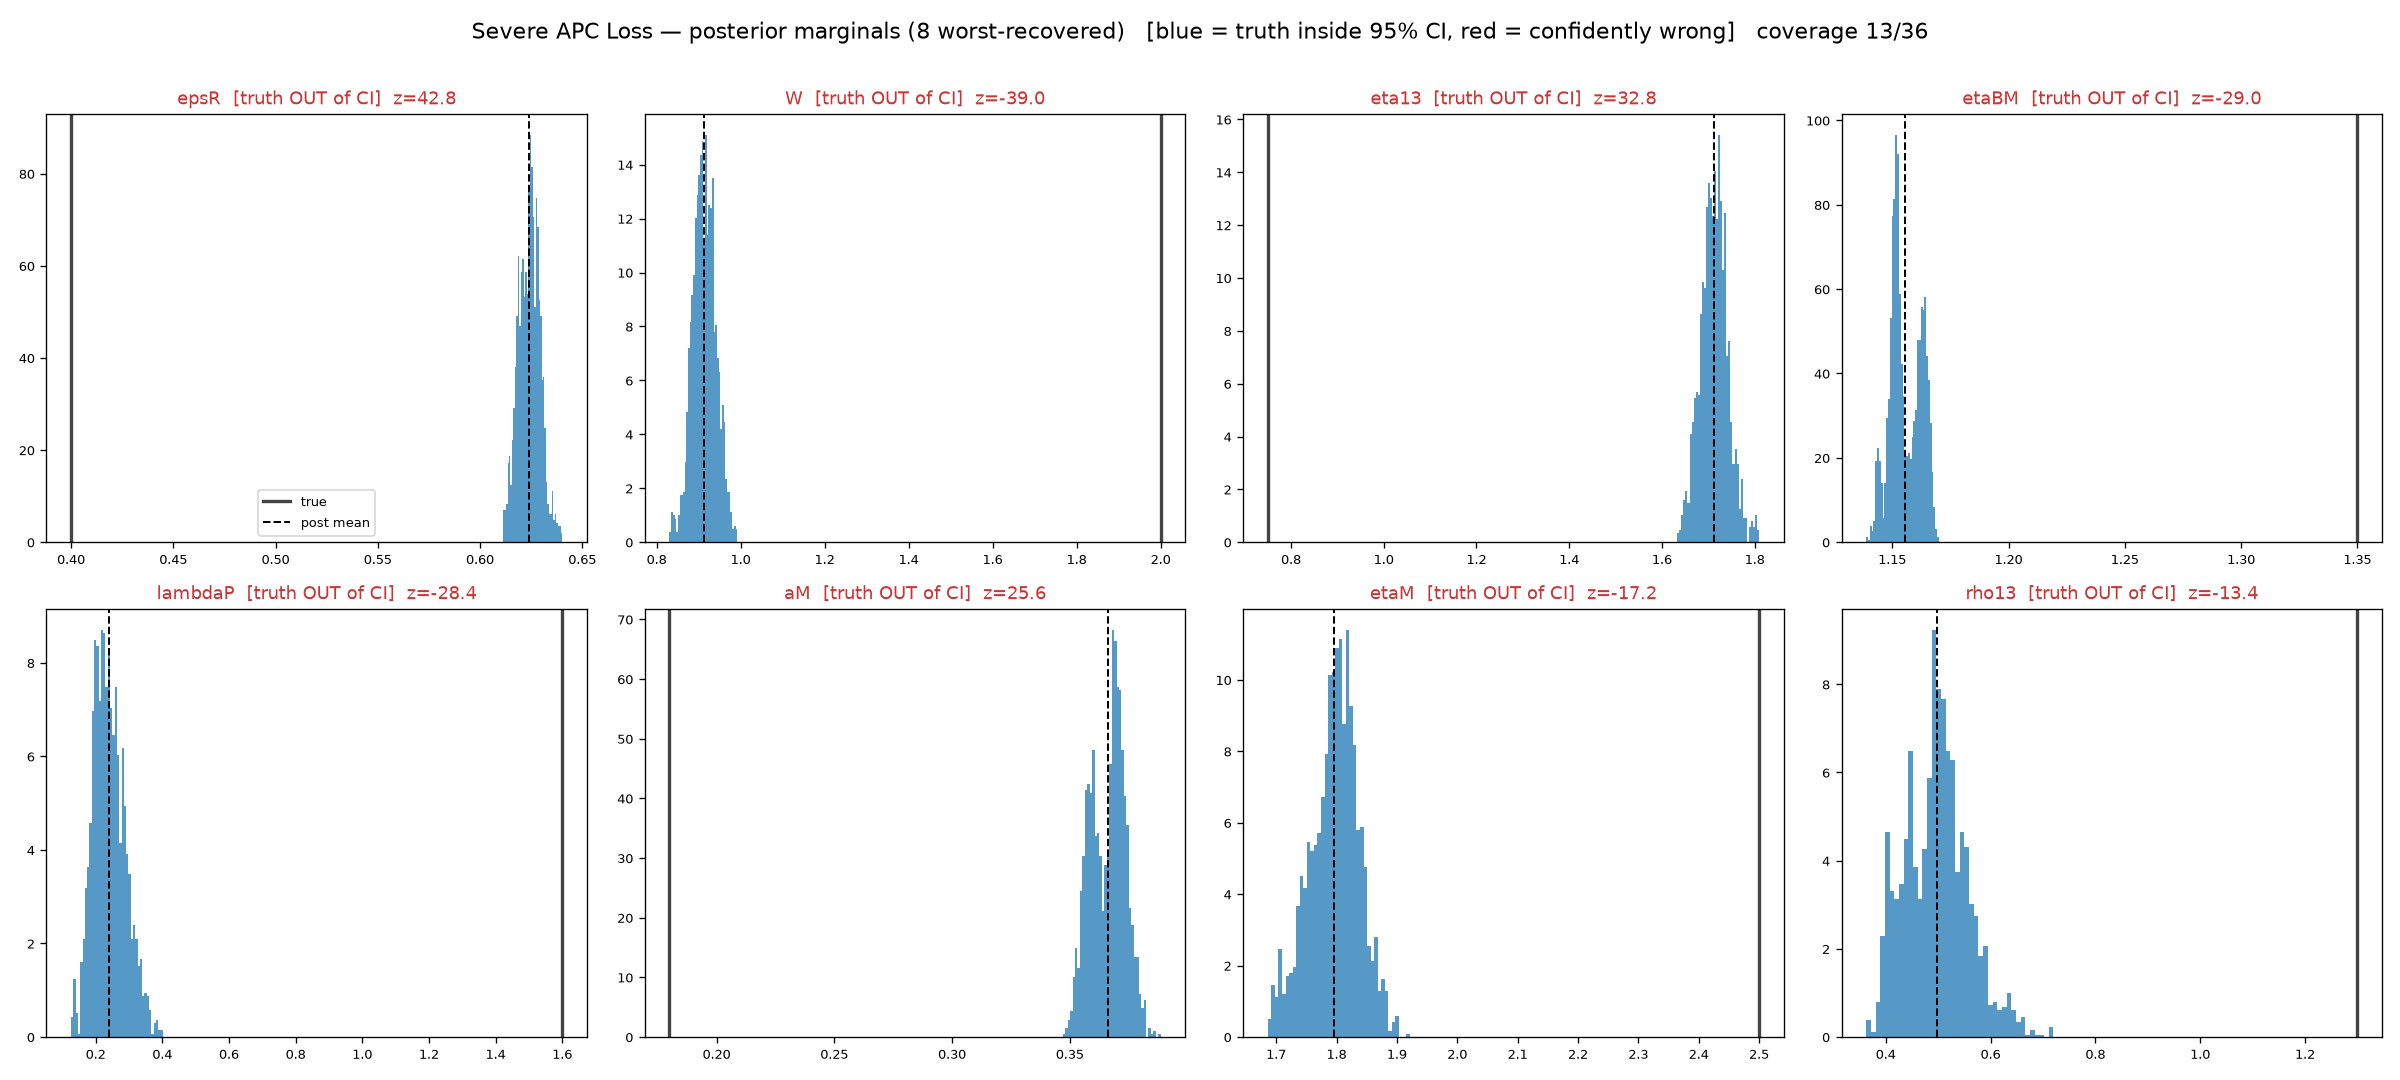
\includegraphics[width=0.96\textwidth]{assets/severe_worst8_marginals.png}
\end{frame}

% 17 — Comparison table
\begin{frame}{Parameter Recovery Comparison}
  \vspace{0.28cm}
  \renewcommand{\arraystretch}{1.52}
  \arrayrulecolor{Cobalt}
  \begin{tabularx}{\textwidth}{@{}Xccc@{}}
    \toprule
    \rowcolor{TintWarm}
    & \textbf{Bayesian inverse PINN} & \textbf{Inverse PINN} & \textbf{ODE-fit} \\
    \midrule
    ``Normal'' & \textcolor{Garnet}{\textbf{19}} & 17 & 18/36 \\
    \rowcolor{Tint}
    ``Early Adenoma'' & \textcolor{Garnet}{\textbf{20}} & 16 & 17/36 \\
    ``Advanced Adenoma'' & \textcolor{Garnet}{\textbf{11}} & 10 & 13/36 \\
    \rowcolor{Tint}
    ``Severe APC Loss'' & \textcolor{Garnet}{\textbf{8}} & 7 & 11/36 \\
    \bottomrule
  \end{tabularx}
  \arrayrulecolor{black}
\end{frame}

% 18 — Next steps
\begin{frame}{Next Steps}
  \begin{columns}[c,totalwidth=\textwidth]
    \begin{column}{0.49\textwidth}
      \begin{itemize}\setlength\itemsep{0.30cm}
        \item Improve Bayesian PINN
          \begin{itemize}\item Investigate limitations\end{itemize}
        \item Hybrid Mechanistic-Neural Model
        \item Stochastic Modeling
      \end{itemize}
    \end{column}
    \begin{column}{0.47\textwidth}
      \centering\imagepanel[width=0.96\linewidth]{assets/source_next_steps.jpg}
    \end{column}
  \end{columns}
\end{frame}

% 19 — References
\begin{frame}[plain]
  \centering
  \vspace{0.24cm}
  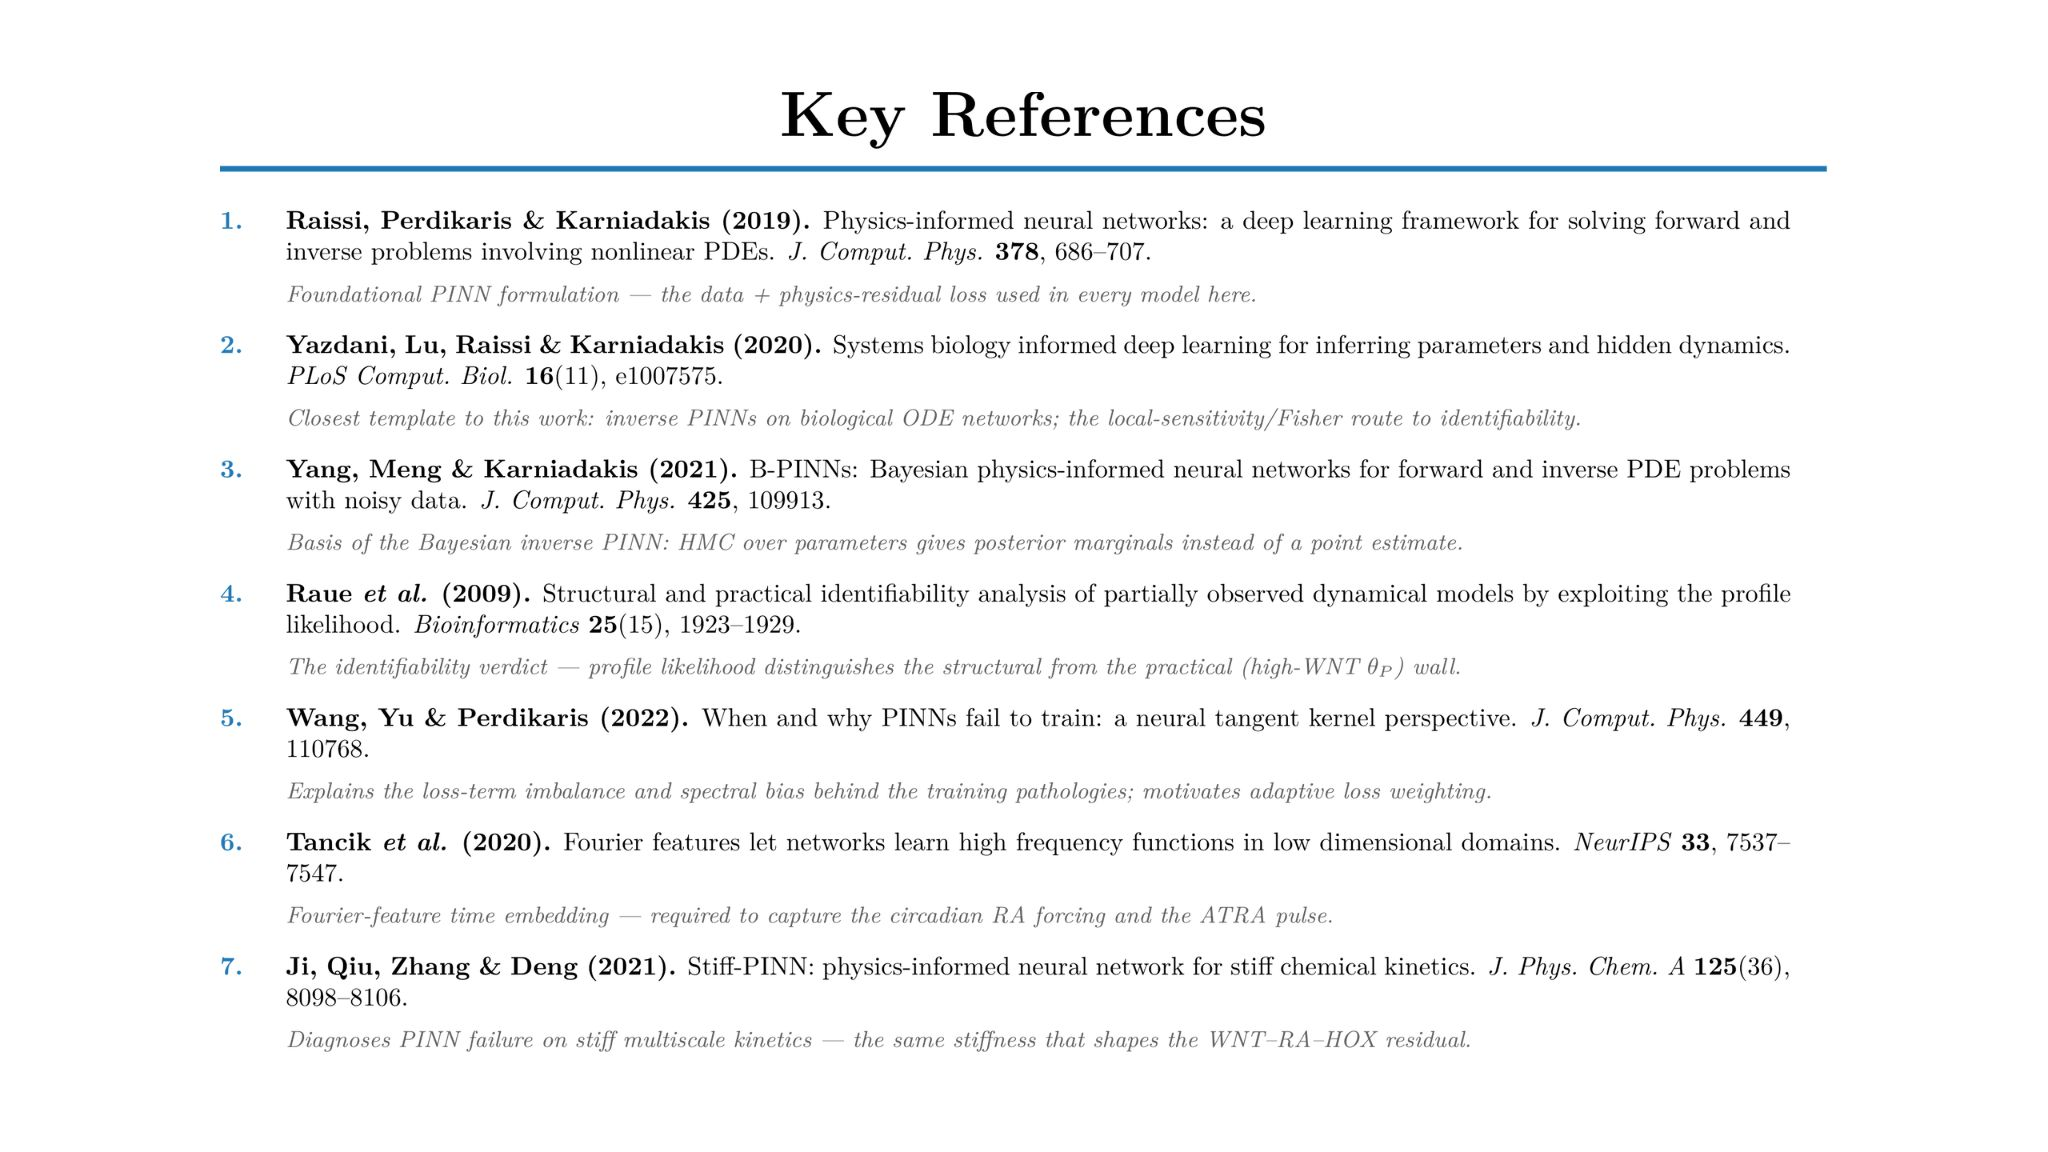
\includegraphics[width=\textwidth]{assets/source_references.jpg}
\end{frame}

% 20 — Thank you
\begin{frame}{Thank you!}
  \centering
  {\large Questions? (we will try to answer)}\hspace{0.14cm}
\includegraphics[height=0.42cm]{assets/source_emoji.jpg}
  \vspace{0.18cm}
  \begin{columns}[T,totalwidth=\textwidth]
    \begin{column}{0.46\textwidth}
      \centering
      {\scriptsize PK calling Amir + Nate to check in on our progress\ldots}\par
      \vspace{0.10cm}
      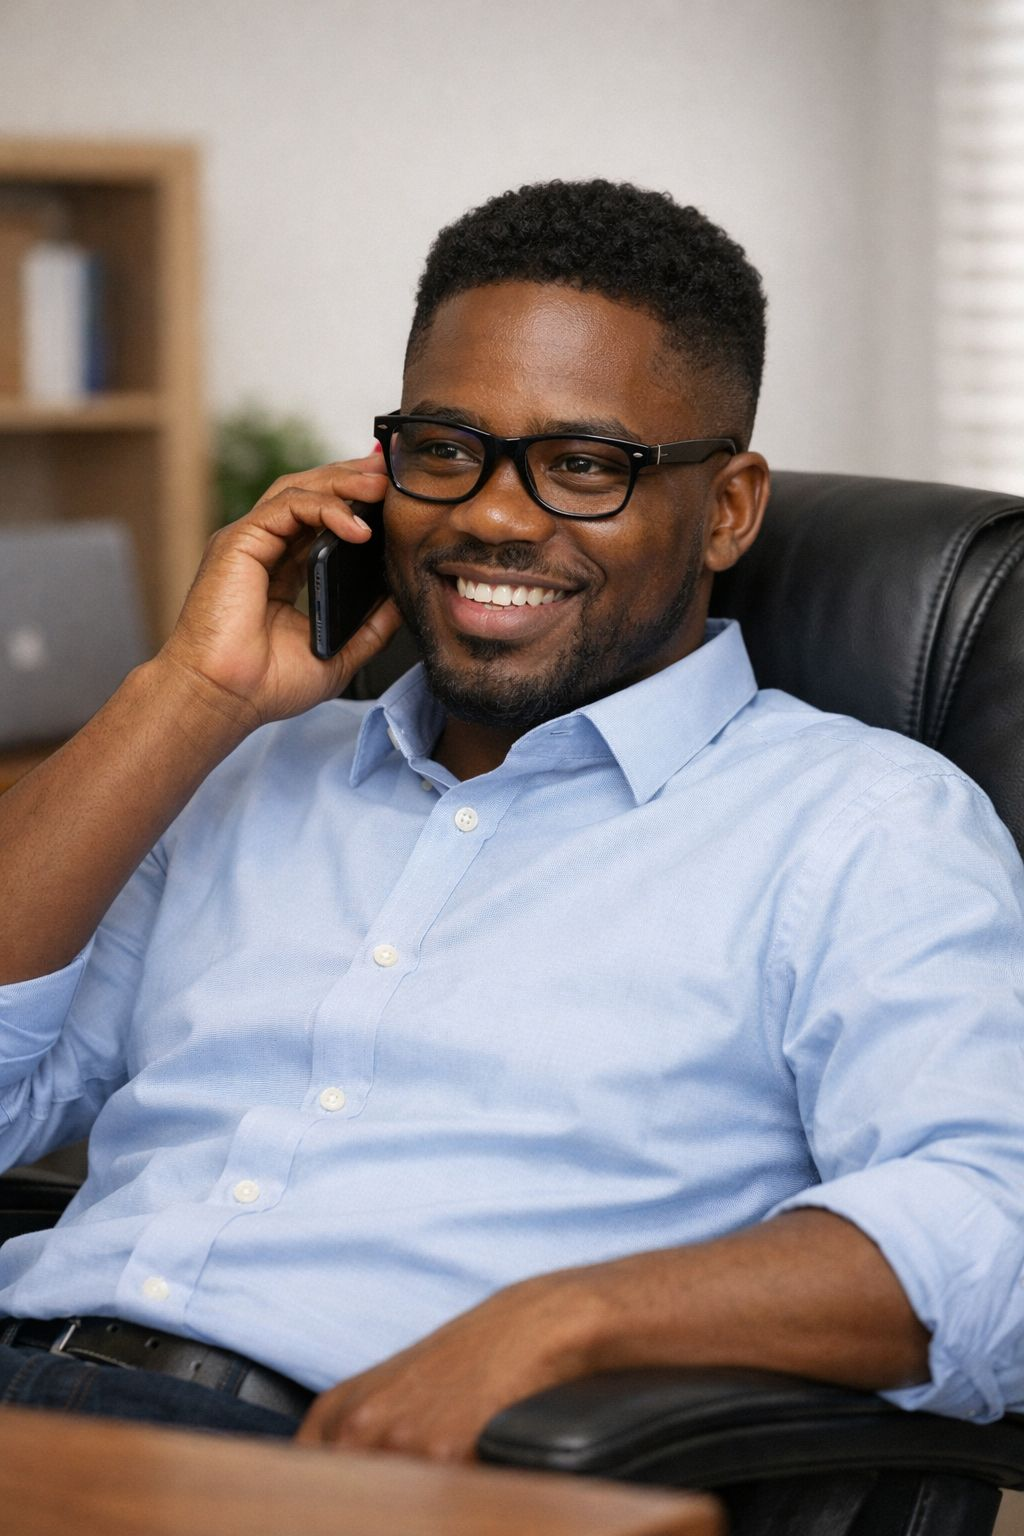
\includegraphics[height=1.35cm]{assets/source_advisor.jpg}
      \vspace{0.12cm}
      \begin{columns}[T,totalwidth=\linewidth]
        \begin{column}{0.49\linewidth}
          \centering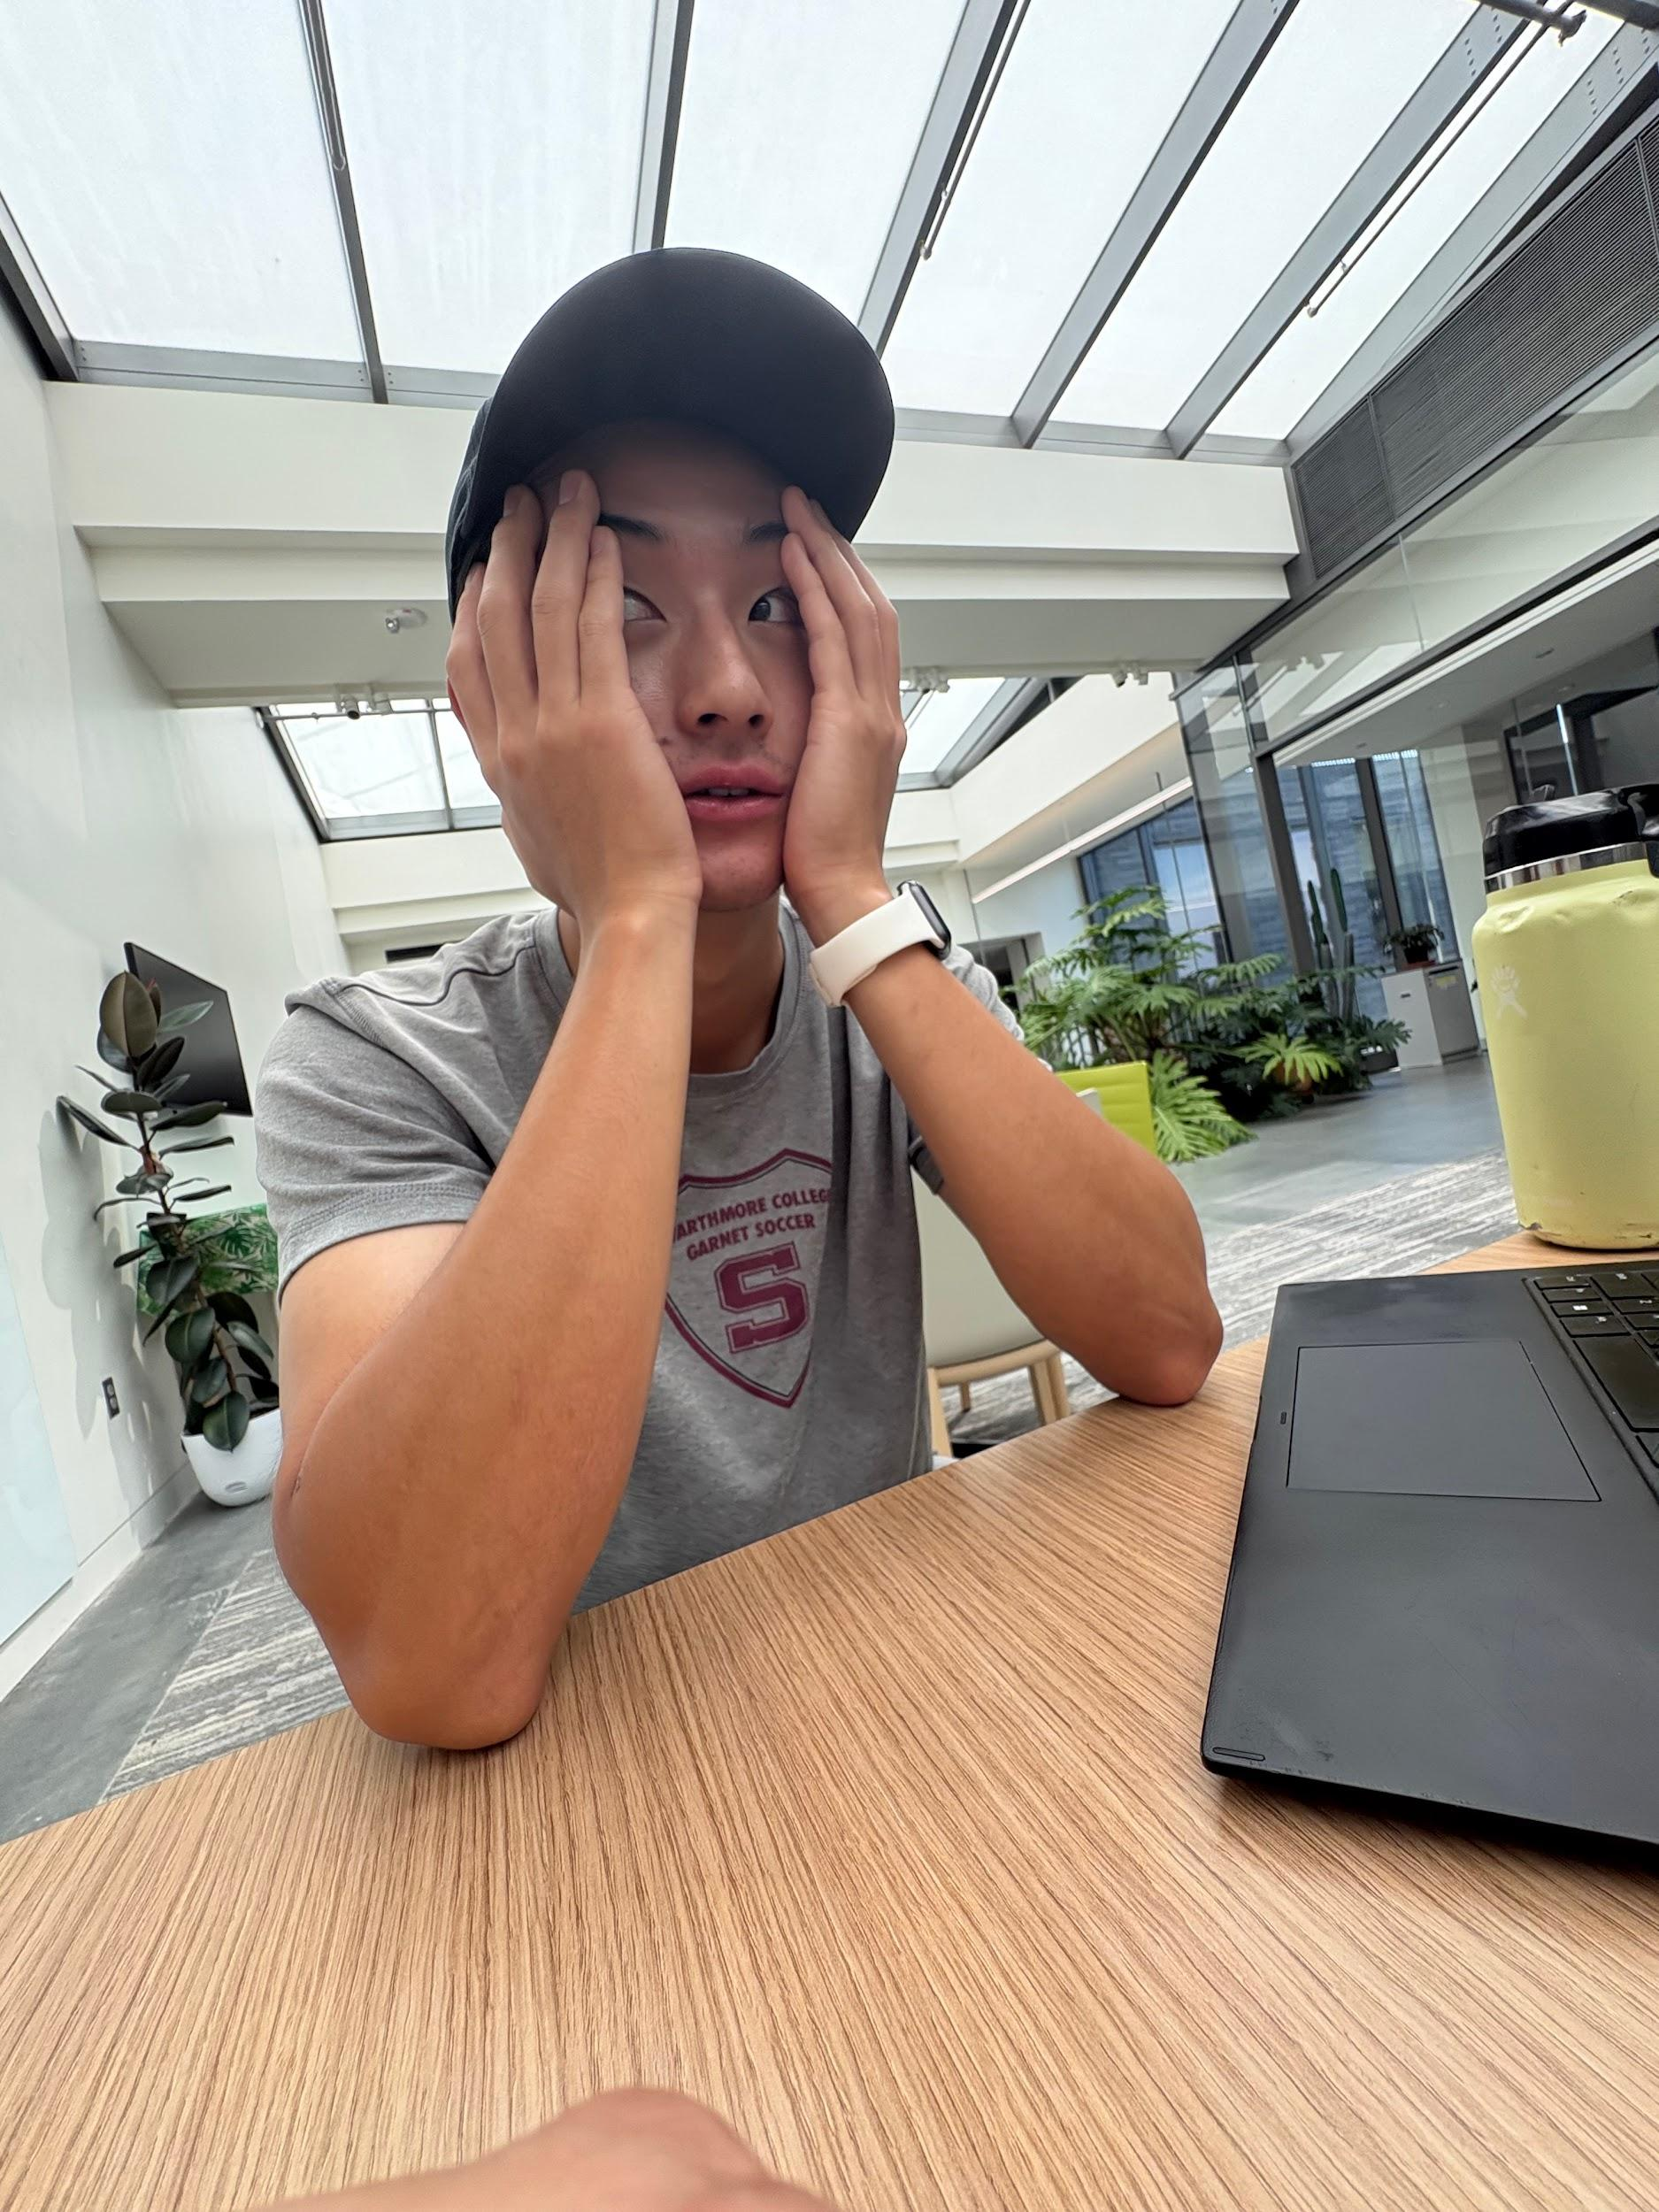
\includegraphics[height=1.95cm]{assets/source_amir.jpg}\par
          {\fontsize{5.2}{6.0}\selectfont 4th diet coke of the day + Celsius b/c his sleep schedule is so cooked}
        \end{column}
        \begin{column}{0.49\linewidth}
          \centering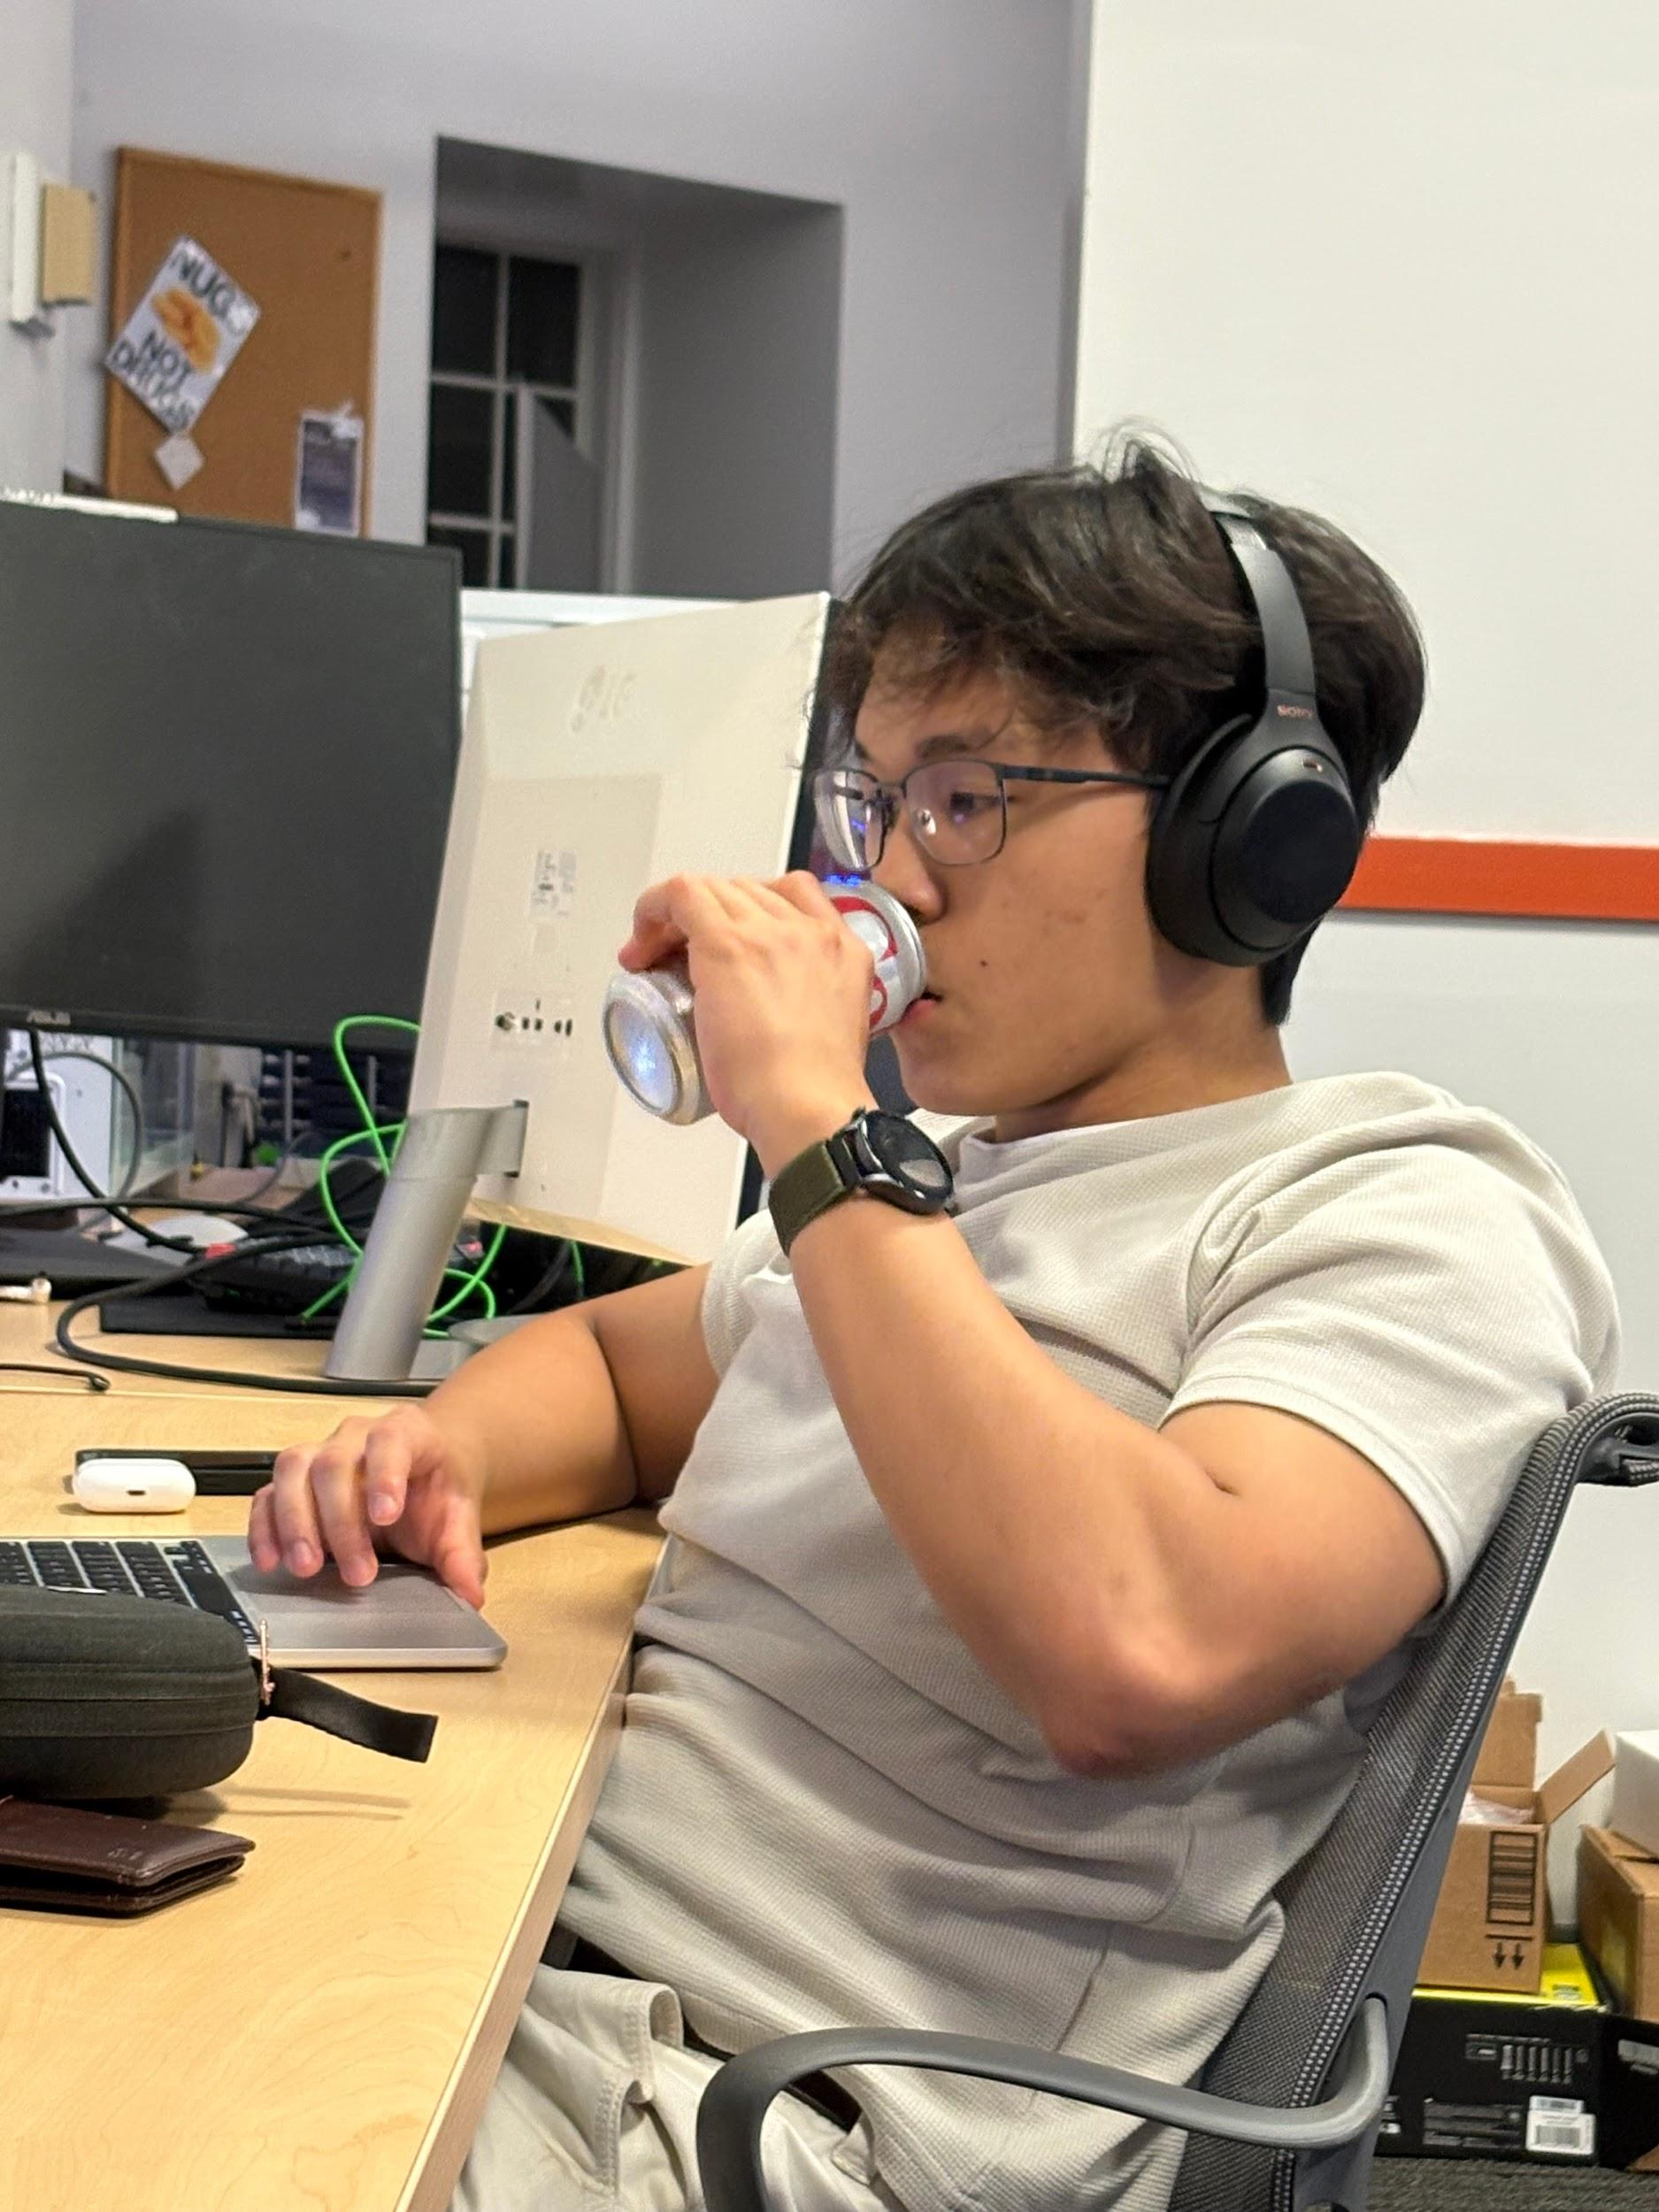
\includegraphics[height=1.95cm]{assets/source_nate.jpg}\par
          {\fontsize{5.2}{6.0}\selectfont Don't know what in the world is going on b/c he spent more hours watching the world cup than working}
        \end{column}
      \end{columns}
    \end{column}
    \begin{column}{0.49\textwidth}
      \centering
      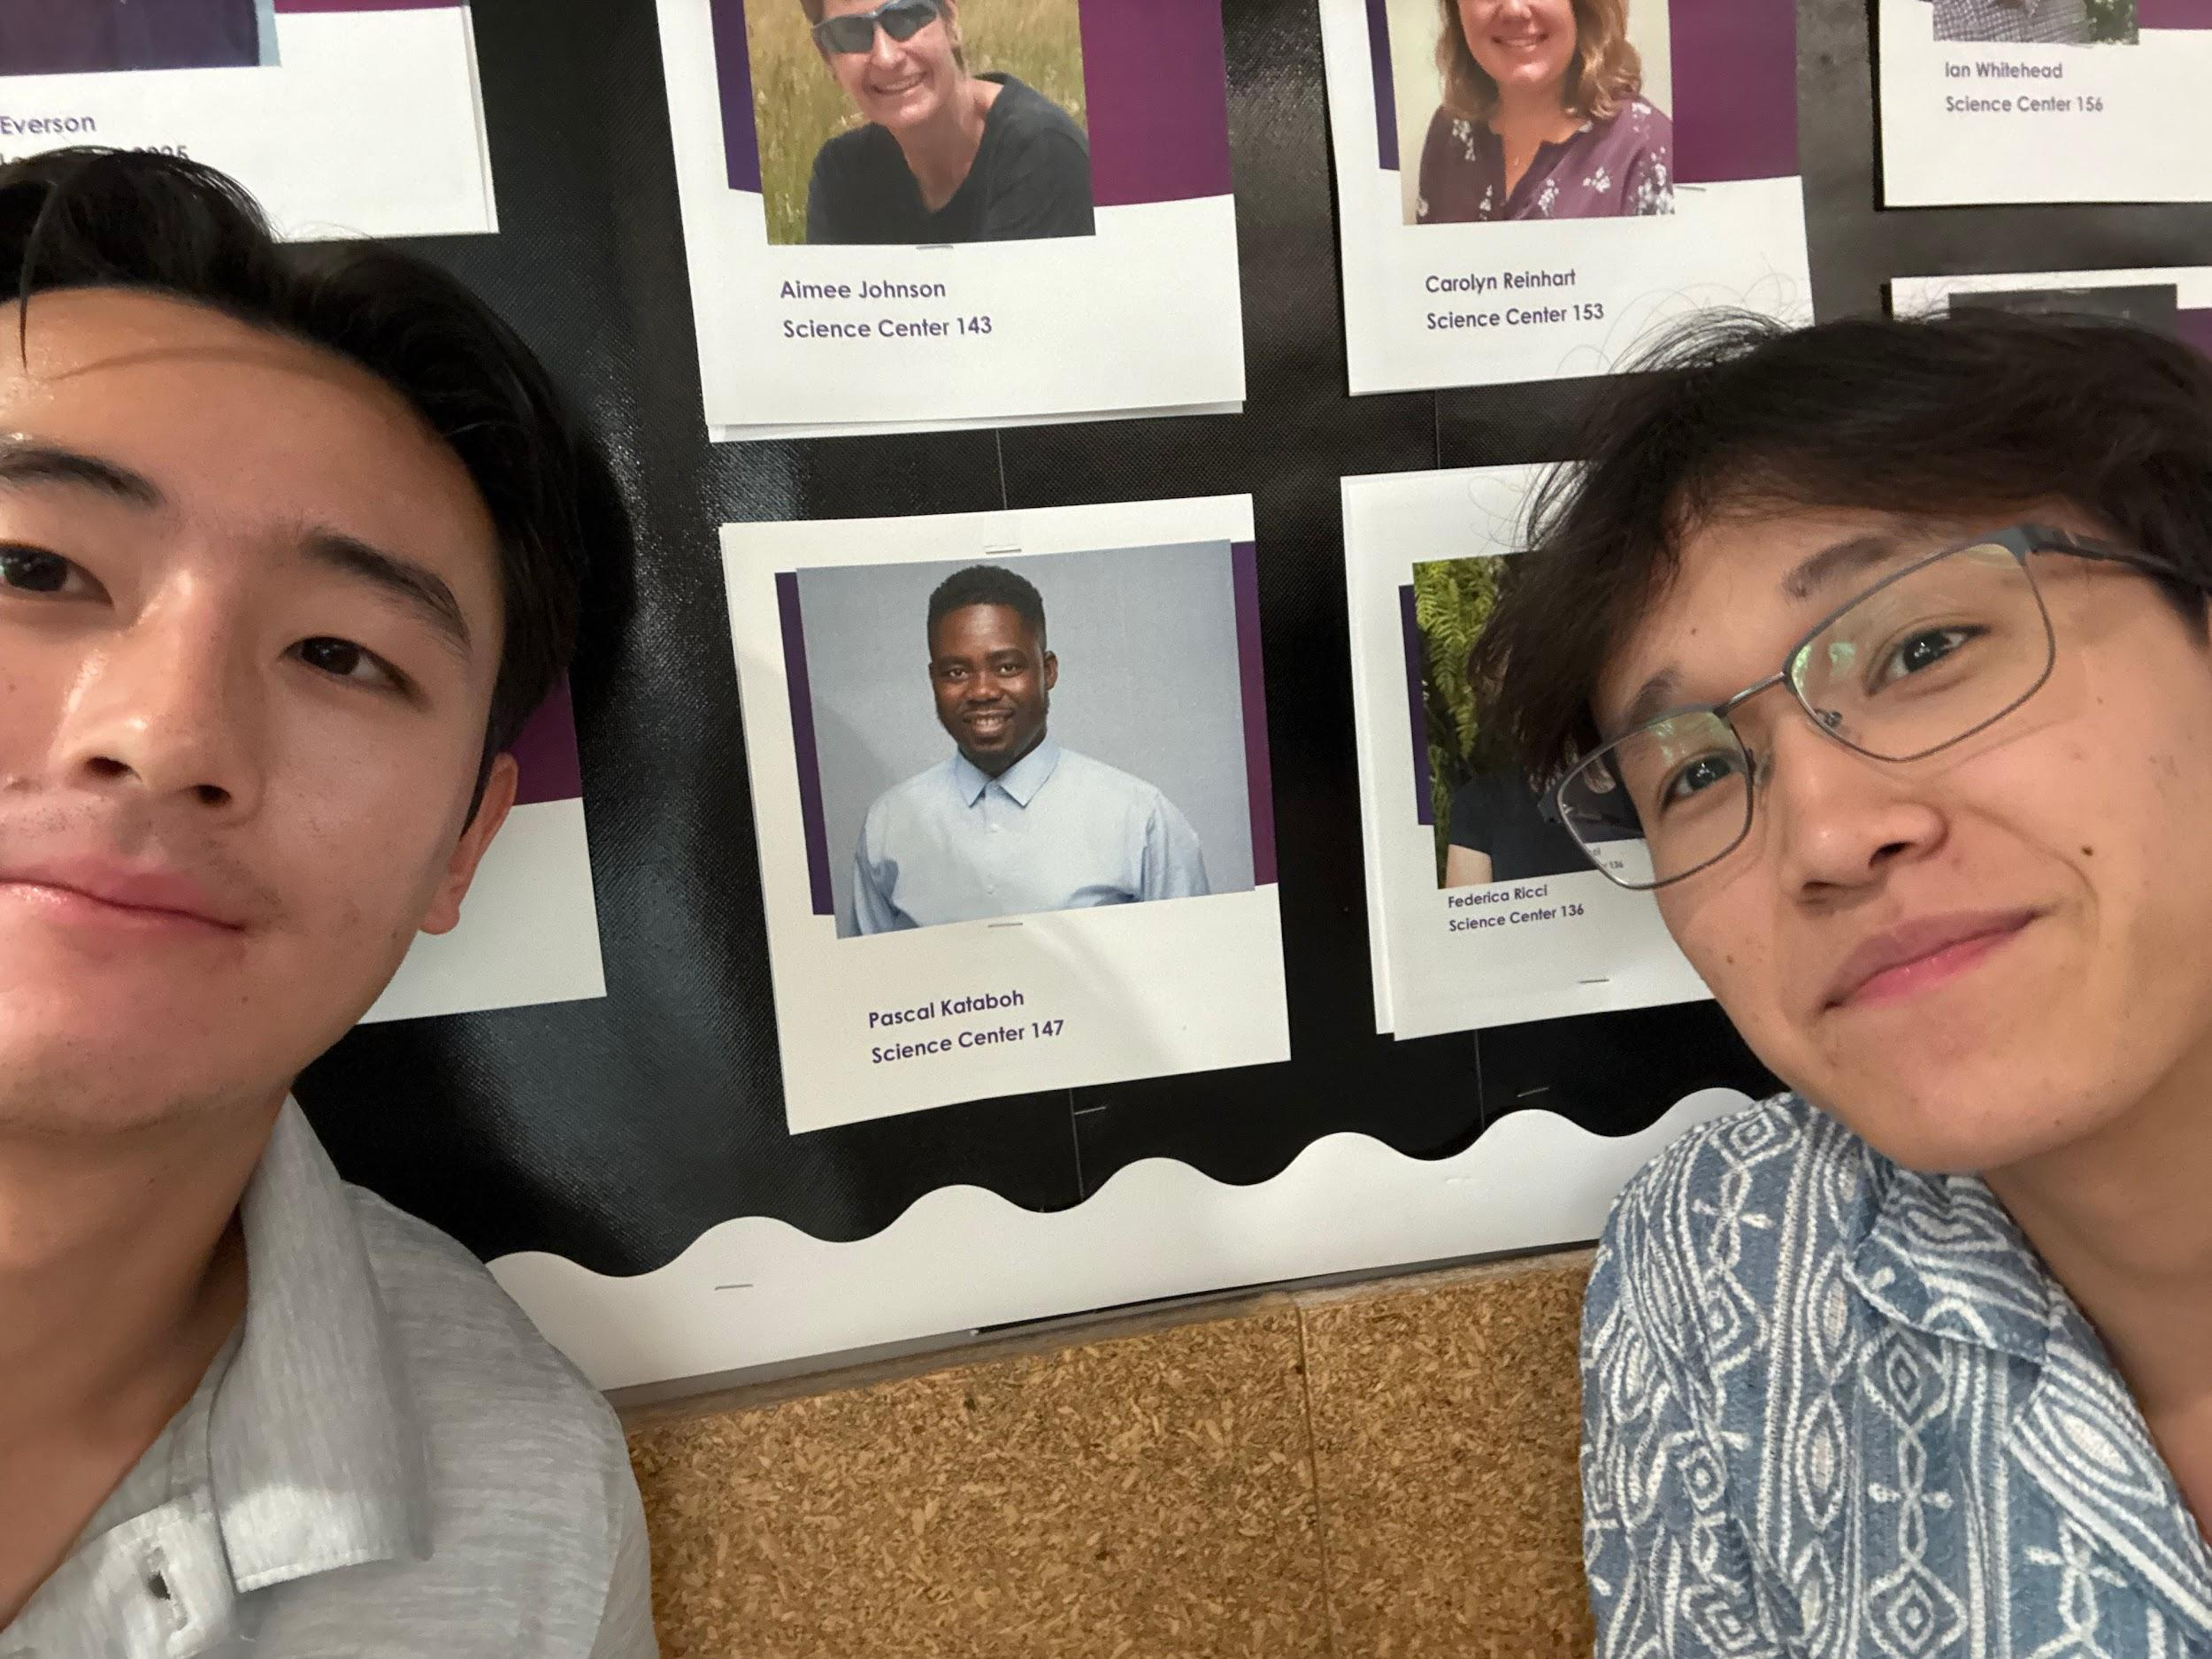
\includegraphics[width=0.92\linewidth]{assets/source_selfie.jpg}\par
      \vspace{0.12cm}
      {\scriptsize Thank you very much to the \textbf{Provost's Office} for funding our summer research project!}
    \end{column}
  \end{columns}
\end{frame}

\end{document}
